
\chapter{\topos{}的范畴论性质}

\philoquote{
    The theory of abelian categories served as the
    ``right'' generalization for the category of abelian groups. So topoi serve for---no less---the category of sets.
}{Peter Freyd, \textit{Aspects of Topoi}}

范畴是一个广泛应用的概念, 然而它的结构比较单薄, 在一般的范畴中能做的事情十分有限. 为了让范畴更有用, 我们就要要求合适的性质. Lawvere 在范畴论的层面研究了这样一个问题: 集合范畴 $\mathsf {Set}$ 具有什么样的性质, 使得它能作为数学的基础. 他将这些性质提炼成为\topos{} (topos) 的概念.

本章的目的是展现集合范畴中的许多构造实际上具有范畴论上的一般性, 也为形式上统一这些构造的 ``\topos{}的内语言'' 埋下伏笔.

\section{范畴论基本概念}

\subsection{极限与余极限}

范畴中常见的极限如下.\footnote{我们假设读者对这些概念有一定的了解, 因此这里仅作一列举.}
\begin{itemize}
    \item \emph{乘积} (product) 是离散图 (若干个无关的对象) 的极限;
    \item \emph{等化子} (equalizer) 是形如 $\begin{tikzcd}[ampersand replacement=\&,sep=small]
	\bullet \& \bullet
	\arrow[shift left=1, from=1-1, to=1-2]
	\arrow[shift right=1, from=1-1, to=1-2]
\end{tikzcd}$ 的图的极限;
    \item \emph{拉回} (pullback) 是形如 $\begin{tikzcd}[ampersand replacement=\&,sep=small]
	\& \bullet \\
	\bullet \& \bullet
	\arrow[from=2-1, to=2-2]
	\arrow[from=1-2, to=2-2]
\end{tikzcd}$ 的图的极限;
    \item \emph{终对象}是空图的极限. 终对象也可视为 $0$ 个对象的积, 因此我们将终对象记作 $1$.
    终对象到另一对象 $c$ 的态射称为 $c$ 的\emph{整体元素} (global element)\footnote{这一称呼来自层的整体截面.}.
\end{itemize}

我们关注的一类极限是\emph{有限图} (有限个对象和有限个态射组成的图) 的极限, 称为\emph{有限极限}. (空图的极限也是一种有限极限.)

范畴中常见的余极限如下.
\begin{itemize}
    \item \emph{二元和}是形如 $\bullet\qquad \bullet$ 的图的余极限;
    \item \emph{余等化子} (coequalizer) 是形如 $\begin{tikzcd}[ampersand replacement=\&,sep=small]
	\bullet \& \bullet
	\arrow[shift left=1, from=1-1, to=1-2]
	\arrow[shift right=1, from=1-1, to=1-2]
\end{tikzcd}$ 的图的余极限;
    \item \emph{推出} (pushout) 是形如 $\begin{tikzcd}[ampersand replacement=\&,sep=small]
	\bullet \& \bullet \\
	\bullet \&
	\arrow[from=1-1, to=2-1]
	\arrow[from=1-1, to=1-2]
\end{tikzcd}$ 的图的余极限;
    \item \emph{始对象}是空图的余极限. 始对象也可视为 $0$ 个对象的和, 因此我们将始对象记作 $0$.
\end{itemize}

使用上面的某些 (余) 极限就可以表达出所有的有限 (余) 极限.

\begin{prop}
    [label={finite-limits-equivalent-condition}]
    {}
    \setlength{\tabcolsep}{12pt}
    \renewcommand{\arraystretch}{1.5}
    \begin{center}
    	\begin{tabular}{l|l}
    		对于范畴 $\mathsf C$, 如下条件等价: \quad & 对于范畴 $\mathsf C$, 如下条件等价: \\
    		(1) 存在有限极限\footnotemark; & (1) 存在有限余极限; \\
    		(2) 存在有限积与等化子; &  (2) 存在有限余积与余等化子;\\
    		(3) 存在终对象与拉回. & (3) 存在始对象与推出.
    	\end{tabular}
    \end{center}
\end{prop}

\footnotetext{``存在有限极限'' 是 ``存在所有的有限极限'' 的简便说法.}

\begin{proof}
    由对偶性, 我们只需证明左边的命题. 由定义, $(1)$ 蕴含 $(2)$ 和 $(3)$.
    
    $(2) \Rightarrow (1)$ 的证明. 设 $F \colon I \to\mathsf C, i\mapsto F_i$ 是任意有限图,
    考虑有限积
    $$
        P = \prod_{i} F_i,\quad
        Q = \prod_{i \to j} F_j
    $$
    (其中下标 $i\to j$ 取遍指标范畴 $I$ 的所有态射) 以及两个态射 $P \to Q$,
    一个是
    $(x_i)_{i} \mapsto (F_{i\to j}(x_i))_{i\to j}$,
    另一个是
    $(x_i)_{i} \mapsto (x_j)_{i\to j}$.
    两个态射的等化子即是极限 $\lim_{i} F_i$.
    注意态射 $P,Q$ 的定义仿佛使用了 ``集合'' 的语言,
    这可以视为一种形式的记号; 无论如何, 它很容易翻译为范畴语言.

    $(3) \Rightarrow (2)$ 的证明.
    到终对象的拉回给出了有限积,
    而对于两个态射 $f,g \colon X \to Y$, 如下拉回给出了等化子:
    % https://q.uiver.app/#q=WzAsNCxbMCwwLCJcXG9wZXJhdG9ybmFtZXtlcX0oZixnKSJdLFsxLDAsIlgiXSxbMCwxLCJYIl0sWzEsMSwiWSJdLFsxLDMsImYiXSxbMiwzLCJnIiwyXSxbMCwyXSxbMCwxXV0=
    \[\begin{tikzcd}[ampersand replacement=\&,column sep=small]
    	{\operatorname{eq}(f,g)} \& Y \\
    	X \& Y\times Y,
    	\arrow["\Delta", from=1-2, to=2-2]
    	\arrow["{(f,g)}"', from=2-1, to=2-2]
    	\arrow[from=1-1, to=2-1]
    	\arrow[from=1-1, to=1-2]
    \end{tikzcd}\]
    其中 $\Delta = (\operatorname{id}_Y,\operatorname{id}_Y) \colon Y\to Y\times Y$ 是\emph{对角线}.
\end{proof}

\subsection{指数对象与积闭范畴}

集合范畴中, 两个集合间的态射仍构成一个集合, 称为映射集合. 在某些范畴 $\mathsf C$ 中, 两个对象之间有一个 $\mathsf C$ 的对象充当了 ``映射集合'' 的角色, 称为\emph{指数对象} (exponential object).

\begin{definition}
    [label={exponential-object}]
    {(指数对象, 积闭范畴)}
    设范畴 $\mathsf C$ 具有有限积. 对固定的对象 $X$, 若存在函子 $(-)^X \colon \mathsf C \to \mathsf C$ 构成 $(-)\times X$ 的右伴随\footnotemark, 即有自然同构
    \begin{equation}
        \operatorname{Hom}_{\mathsf C}(Z,Y^X)  \simeq \operatorname{Hom}_{\mathsf C}(Z\times X,Y),
        \label{exponential-adjoint}
    \end{equation}
    则称 $X$ \emph{可作指数} (exponentiable), 称 $Y^X$ 为\emph{指数对象} (exponential object), 或称\emph{内蕴态射对象} (internal hom-object).
    
    若 $\mathsf C$ 的所有对象均可作指数, 则称 $\mathsf C$ 为\emph{积闭范畴} (cartesian closed category), 其中 ``闭'' 即指数对象的存在性.
\end{definition}

\footnotetext{指数对象可对一般的\emph{幺半范畴} (monoidal category) 定义, 这里我们只考虑所谓\emph{积幺半范畴} (cartesian monoidal category), 即以乘积定义的幺半范畴.}

指数对象在数学中随处可见.

\begin{example}
    {(紧开拓扑)}
    在拓扑空间范畴 $\mathsf {Top}$ 中, 一般的对象不一定可作指数, 但局部紧 Hausdorff 空间都是可作指数的.
    若 $X$ 是局部紧空间, $Y$ 是任意拓扑空间,
    指数对象 $Y^X$ 上的拓扑称为\emph{紧开拓扑} (compact-open topology),
    这个名字是因为它可由如下开集生成:
    对紧集 $K\subset X$ 与开集 $O\subset Y$,
    取 $X$ 到 $Y$ 所有满足 $f(K) \subset O$ 的映射构成的集合.
    
    拓扑学中, 人们常说 ``我们在一个方便的拓扑空间范畴中工作''\footnotemark,
    即要求所考虑的范畴包含我们感兴趣的空间, 且具有积闭等性质.
    一个比较方便的范畴是\emph{紧生成弱 Hausdorff 空间范畴} $\mathsf{CGWH}$. Johnstone \cite{Johnstone-OTT} 构造了一个方便的拓扑空间范畴, 且它是\topos{}.
\end{example}
\footnotetext{\url{https://ncatlab.org/nlab/show/convenient+category+of+topological+spaces}}

\begin{example}
    {(函子范畴)}
    两个范畴 $\mathsf C,\mathsf D$ 之间的函子构成一个范畴 $\mathsf {Fun}(\mathsf C,\mathsf D)$, 这是范畴的范畴 $\mathsf {Cat}$ 中的指数对象.
\end{example}

\begin{prop}
    {}
    对于积闭范畴, 指数对象实际上构成一个\emph{双函子} (也即乘积范畴出发的函子) $\mathsf C^{\op}\times\mathsf C \to \mathsf C$, $(X,Y)\mapsto Y^X$.
\end{prop}

    %指数对象的性质也可表述为函子 . 下面 (\ref{slice-category} 节) 还会介绍更多相关的性质.
    
    %另外, 即使范畴中没有乘积也可定义指数对象: 使用米田嵌入 $\yo \colon \mathsf C \to \mathsf {Fun}(\mathsf C^{\op},\mathsf {Set})$,
    %指数对象 $Y^X$ 是函子 $\yo(Y)^{\yo(X)}$ 的表示对象.

    

在集合范畴中, 给定一个映射 $f\colon X\to Y$ 与一个元素 $x\in X$, 我们可对 $f$ 在 $x$ 处取值得到 $Y$ 的元素 $f(x)$; 类似地, 在一个积闭范畴中我们有 $Y^X\times X$ 到 $Y$ 的一个 ``取值'' 映射.

\begin{definition}
    [label={evaluation-map}]
    {(取值映射)}
    在 (\ref{exponential-adjoint}) 中取 $Z=Y^X$, 那么 $\operatorname{id}_{Y^X}\in \operatorname{Hom}_{\mathsf C}(Y^X,Y^X)$ 在另一边对应的态射称作\emph{取值映射} (evaluation map) $\operatorname{ev}\colon Y^X\times X \to Y$. 换言之, 取值映射 $\operatorname{ev}\colon Y^X\times X \to Y$ 是伴随 $(-)\times X \dashv (-)^X$ 的余单位.
\end{definition}

指数对象有与数的乘方类似的规律.

\begin{prop}
	[label={exponential-law}]
	{(指数律)}
	在积闭范畴中, 对任意对象 $X,Y,Z$ 有
	$$
	(Z^{Y})^X\simeq Z^{Y\times X}.
	$$
\end{prop}

\begin{proof}
	由指数对象的性质, 有自然同构
	\begin{align*}
		\operatorname{Hom}(W,(Z^{Y})^X)
		&\simeq\operatorname{Hom}(W\times X,Z^Y)\\
		&\simeq\operatorname{Hom}(W\times X\times Y,Z)\simeq\operatorname{Hom}(W,Z^{Y\times X}).
	\end{align*}
	由米田引理, 结论得证.
\end{proof}

\begin{prop}
	[label={sum-exponential-product}]
	{}
	在有二元和的积闭范畴中, 对任意对象 $X,Y,Z$ 有
	$$
	Z^{X + Y}\simeq Z^X \times Z^Y.
	$$
\end{prop}

\begin{proof}
	略. 与命题 \ref{exponential-law} 的证明类似, 使用米田引理.
%	\begin{align*}
%		\operatorname{Hom}(W,Z^{X+Y})
%		&\simeq\operatorname{Hom}(W\times (X+Y),Z)\\
%		&\simeq\operatorname{Hom}(W\times X+W\times Y,Z)\\
%		&\simeq\operatorname{Hom}(W\times X,Z)+\operatorname{Hom}(W\times Y,Z)\\
%		&\simeq\operatorname{Hom}(W,Z^X)\times\operatorname{Hom}(W,Z^Y)\\
%		&\simeq\operatorname{Hom}(W,Z^X\times Z^Y).
%	\end{align*}
	其中要用到积闭范畴中的 ``分配律'' $$W\times (X+Y)\simeq W\times X+W\times Y,$$ 这是因为 $(-)\times W$ 作为 $(-)^W$ 的左伴随保持余极限 (命题 \ref{adjoints-preserve-limits}).
\end{proof}


\begin{prop}
	[label={product-exponential-product}]
	{}
	在积闭范畴中,
	$$
	(Z\times Y)^X\simeq Z^X\times Y^X.
	$$
\end{prop}

\begin{proof}
	这是因为 $(-)^X$ 作为 $(-)\times X$ 的右伴随保持极限 (命题 \ref{adjoints-preserve-limits}).
\end{proof}

\subsection{子对象分类子}

对于集合 $X$ 的子集 $U\subset X$,
定义其\emph{特征函数} (characteristic function) $\chi_U \colon X \to \{0,1\}$,
$$
\chi_U(x) = \begin{cases}
    \ 1, & x\in U,\\
    \ 0, & x\notin U.
\end{cases}
$$
(我们可将特征函数 $\chi_U(x)$ 视为 ``含一个变量 $x$ 的命题'', 当且仅当 $x\in U$ 时命题为真.)
如此, $X$ 的子集一一对应于 $X$ 到 $\{0,1\}$ 的映射.
这就是说, 集合 $\{0,1\}$ ``分类'' (classify) 了集合的子集.

\begin{definition}
    {(子对象)}
    在一般的范畴中, 我们称指向 $X$ 的单态射 $U \to X$ \emph{的同构类}为 $X$ 的\emph{子对象} (subobject), 其中单态射的同构是指形如
    % https://q.uiver.app/#q=WzAsMyxbMCwwLCJVIl0sWzAsMiwiXFx3aWRldGlsZGUgVSJdLFsxLDEsIlgiXSxbMCwyLCIiLDAseyJzdHlsZSI6eyJ0YWlsIjp7Im5hbWUiOiJob29rIiwic2lkZSI6InRvcCJ9fX1dLFsxLDIsIiIsMix7InN0eWxlIjp7InRhaWwiOnsibmFtZSI6Imhvb2siLCJzaWRlIjoiYm90dG9tIn19fV0sWzAsMSwiXFxzaW1lcSIsMix7Im9mZnNldCI6MX1dLFsxLDAsIiIsMSx7Im9mZnNldCI6MX1dXQ==
    $\begin{tikzcd}[ampersand replacement=\&,row sep=-1pt]
    	U \\
    	\& X \\
    	{\widetilde U}
    	\arrow[hook, from=1-1, to=2-2]
    	\arrow[hook', from=3-1, to=2-2]
    	\arrow["\simeq"', shift right=1, from=1-1, to=3-1]
    	\arrow[shift right=1, from=3-1, to=1-1]
    \end{tikzcd}$
    的交换图.
\end{definition}



范畴 $\mathsf C$ 中对象 $X$ 的子对象构成一偏序集 $\operatorname{Sub}_{\mathsf C}(X)$, 其序关系为 ``包含'' 关系. 若子对象 $U\hookrightarrow X$ 作为嵌入映射可分解为 $U\hookrightarrow V \hookrightarrow X$, 则称 $U$ 包含于 $V$.
%这个偏序集作为范畴, 其中的乘积为子对象的\emph{交}.

在范畴 $\mathsf C$ 具有拉回时, 子对象集合有函子性.

\begin{definition}{(子对象函子)}
    假设范畴 $\mathsf C$ 具有拉回. 定义\emph{子对象函子}
    $$\operatorname{Sub}_{\mathsf C} \colon \mathsf C^{\op} \to \mathsf {Set},$$
    将对象 $X$ 对应到其子对象的集合,
    态射对应到子对象的拉回.
\end{definition}

上述定义的合法性来自如下命题.

\begin{prop}{}
    在任何范畴中拉回保持子对象; 即对任意态射 $f \colon X \to Y$ 以及子对象 $i \colon V \to Y$, 只要存在拉回 $U = X\times_{Y} V$, 就有 $j=f^* i\colon U\to X$ 是 $X$ 的子对象.
    % https://q.uiver.app/#q=WzAsNCxbMCwxLCJYIl0sWzEsMSwiWSJdLFsxLDAsIlYiXSxbMCwwLCJVIl0sWzAsMSwiZiIsMl0sWzMsMCwiaiIsMix7InN0eWxlIjp7InRhaWwiOnsibmFtZSI6Imhvb2siLCJzaWRlIjoiYm90dG9tIn19fV0sWzMsMiwicCJdLFsyLDEsImkiLDAseyJzdHlsZSI6eyJ0YWlsIjp7Im5hbWUiOiJob29rIiwic2lkZSI6ImJvdHRvbSJ9fX1dXQ==
\[\begin{tikzcd}[ampersand replacement=\&]
	U \& V \\
	X \& Y
	\arrow["f"', from=2-1, to=2-2]
	\arrow["j"', hook', from=1-1, to=2-1]
	\arrow["p", from=1-1, to=1-2]
	\arrow["i", hook', from=1-2, to=2-2]
\end{tikzcd}\]
\end{prop}
\begin{proof}
    设 $j$ 余等化 $\alpha,\beta \colon Z \to U$.% 满足 $j \alpha = j \beta$.
    那么 $fj=ip$ 也余等化 $\alpha,\beta$.
    由 $i$ 为单态射, 知 $p$ 余等化 $\alpha,\beta$.
    由拉回的性质, 知 $\alpha = \beta$.
    这说明 $j$ 为单射.
\end{proof}


\begin{definition}[label={Subobject-classifier-definition}]{(子对象分类子)}
    设范畴 $\mathsf C$ 存在拉回. 若子对象函子 $\operatorname{Sub} \colon \mathsf C^{\op} \to \mathsf {Set}$ 可表, 即存在对象 $\Omega$ 使得有自然同构
    $$
    \operatorname{Sub}_{\mathsf C}(X) \simeq \operatorname{Hom}_{\mathsf C}(X,\Omega),
    $$
    则称 $\Omega$ 为 $\mathsf C$ 的\emph{子对象分类子} (subobject classifier).
\end{definition}

子对象分类子还有如下的等价定义.

\begin{definition}[label={Subobject-classifier-definition-alternative}]{(子对象分类子, 等价定义)}
    设范畴 $\mathsf C$ 存在拉回以及终对象 $1$. 若存在满足如下条件的对象 $\Omega$ 以及单射 $\top \colon 1 \to \Omega$, 则称其为 $\mathsf C$ 的\emph{子对象分类子} (subobject classifier): 对任意单射 (子对象) $U \to X$ 存在唯一的\emph{特征函数} (characteristic map) $\chi_U \colon X \to \Omega$ 使得下图为拉回.
    % https://q.uiver.app/#q=WzAsNCxbMCwwLCJVIl0sWzAsMSwiWCJdLFsxLDAsIjEiXSxbMSwxLCJcXE9tZWdhIl0sWzEsMywiXFxjaGlfVSIsMl0sWzAsMSwiIiwwLHsic3R5bGUiOnsidGFpbCI6eyJuYW1lIjoiaG9vayIsInNpZGUiOiJib3R0b20ifX19XSxbMiwzLCJcXHRvcCIsMCx7InN0eWxlIjp7InRhaWwiOnsibmFtZSI6Imhvb2siLCJzaWRlIjoiYm90dG9tIn19fV0sWzAsMl1d
    \[\begin{tikzcd}[ampersand replacement=\&]
    	U \& 1 \\
    	X \& \Omega
    	\arrow["{\chi_U}"', from=2-1, to=2-2]
    	\arrow[hook', from=1-1, to=2-1]
    	\arrow["\top", hook', from=1-2, to=2-2]
    	\arrow[from=1-1, to=1-2]
    \end{tikzcd}\]
    我们也称 $\top \colon 1 \to \Omega$ 为\emph{万有子对象} (universal subobject).
\end{definition}

有了子对象分类子, 子对象等同于到 $\Omega$ 的态射, 从而子对象的拉回不过是到 $\Omega$ 的态射的复合.
% https://q.uiver.app/#q=WzAsNixbMCwxLCJYIl0sWzEsMSwiWSJdLFsyLDEsIlxcT21lZ2EiXSxbMiwwLCIxIl0sWzEsMCwiViJdLFswLDAsImZeKlYiXSxbNSwwLCIiLDAseyJzdHlsZSI6eyJ0YWlsIjp7Im5hbWUiOiJob29rIiwic2lkZSI6ImJvdHRvbSJ9fX1dLFswLDEsImYiLDJdLFsxLDJdLFs1LDRdLFs0LDNdLFszLDIsIlxcdG9wIl0sWzQsMSwiIiwxLHsic3R5bGUiOnsidGFpbCI6eyJuYW1lIjoiaG9vayIsInNpZGUiOiJib3R0b20ifX19XV0=
\[\begin{tikzcd}[ampersand replacement=\&]
	{f^*V} \& V \& 1 \\
	X \& Y \& \Omega
	\arrow[hook', from=1-1, to=2-1]
	\arrow["f"', from=2-1, to=2-2]
	\arrow[from=2-2, to=2-3]
	\arrow[from=1-1, to=1-2]
	\arrow[from=1-2, to=1-3]
	\arrow["\top", from=1-3, to=2-3]
	\arrow[hook', from=1-2, to=2-2]
\end{tikzcd}\]

\begin{remark}{}
    ``万有子对象'' 中的 ``万有'' 与拓扑学中 ``万有 $G$-主丛'' 中 ``万有'' 的含义相同.

    上述定义中 ``$1$ 是终对象'' 的要求可不用提, 因为它蕴含于后面的泛性质中: 对任何对象 $X$ 考虑子对象 $\operatorname{id}\colon X \to X$, 在拉回图
    % https://q.uiver.app/#q=WzAsNCxbMCwwLCJYIl0sWzAsMSwiWCJdLFsxLDEsIlxcT21lZ2EiXSxbMSwwLCJcXHdpZGV0aWxkZSAxIl0sWzAsMSwiXFxvcGVyYXRvcm5hbWV7aWR9IiwyXSxbMCwzLCJcXGFscGhhIl0sWzEsMiwiXFxjaGkiLDJdLFszLDIsIlxcdG9wIl1d
    $\begin{tikzcd}[ampersand replacement=\&,sep=small]
	X \& {\widetilde 1} \\
	X \& \Omega
	\arrow["{\operatorname{id}}"', from=1-1, to=2-1]
	\arrow["\alpha", from=1-1, to=1-2]
	\arrow["\chi"', from=2-1, to=2-2]
	\arrow["\top", from=1-2, to=2-2]
    \end{tikzcd}$
    中, 由 $\chi$ 的唯一性以及 $\top$ 是单射可得到 $\alpha$ 的唯一性, 这说明 $\widetilde 1$ 就是\makebox{终对象 $1$.}
    
    符号 $\top$ (\LaTeX 代码: \verb|\top|) 读作 ``真'', 后面也将用到另一个元素 $\bot\colon 1\to\Omega$ (\verb|\bot|), 读作 ``假''. 一般地, 态射 $1\to\Omega$ 称为\emph{真值} (truth value).
\end{remark}

现在证明子对象分类器两种定义的等价性. 假设第一种定义 (\ref{Subobject-classifier-definition}) 中的对象 $\Omega$ 存在, 我们需要给出第二种定义 (\ref{Subobject-classifier-definition-alternative}) 所要求的单射 $\top\colon 1 \to \Omega$.

考虑 $\Omega$ 到自身的恒等映射 $\operatorname{id}\colon \Omega \to \Omega$, 它在同构 $\operatorname{Sub}(\Omega) \simeq \operatorname{Hom}(\Omega,\Omega)$ 下对应一个子对象 $\widetilde \top \colon \widetilde 1 \to \Omega$.

对任意子对象 $U\to X$, 由交换图
\[\begin{tikzcd}[ampersand replacement=\&]
	{\widetilde 1} \& {\operatorname{Sub}(\Omega)} \& {\operatorname{Hom}(\Omega,\Omega)} \& {\operatorname{id}_{\Omega}} \\
	U \& {\operatorname{Sub}(X)} \& {\operatorname{Hom}(X,\Omega)} \& {\chi_U}
	\arrow["\ni"{marking}, draw=none, from=1-4, to=1-3]
	\arrow["\simeq", <->, from=1-2, to=1-3]
	\arrow["\simeq"', <->, from=2-2, to=2-3]
	\arrow["\in"{marking}, draw=none, from=1-1, to=1-2]
	\arrow["\in"{marking}, draw=none, from=2-1, to=2-2]
	\arrow["\ni"{marking}, draw=none, from=2-4, to=2-3]
	\arrow["{\text{沿 $\chi_U$ 拉回}}"', from=1-2, to=2-2]
	\arrow["{\text{复合 $\chi_U$}}", from=1-3, to=2-3]
\end{tikzcd}\]
我们得到
% https://q.uiver.app/#q=WzAsNCxbMCwwLCJVIl0sWzAsMSwiWCJdLFsxLDAsIlxcd2lkZXRpbGRlIDEiXSxbMSwxLCJcXE9tZWdhIl0sWzAsMSwiIiwwLHsic3R5bGUiOnsidGFpbCI6eyJuYW1lIjoiaG9vayIsInNpZGUiOiJib3R0b20ifX19XSxbMiwzLCJ0IiwwLHsic3R5bGUiOnsidGFpbCI6eyJuYW1lIjoiaG9vayIsInNpZGUiOiJib3R0b20ifX19XSxbMSwzLCJcXGNoaV9VIiwyXSxbMCwyXV0=
$\begin{tikzcd}[ampersand replacement=\&,sep=small]
	U \& {\widetilde 1} \\
	X \& \Omega
	\arrow[hook', from=1-1, to=2-1]
	\arrow["{\widetilde \top}", hook', from=1-2, to=2-2]
	\arrow["{\chi_U}"', from=2-1, to=2-2]
	\arrow[from=1-1, to=1-2]
\end{tikzcd}$
是一个拉回. 这说明 $\widetilde \top$ 就是 $\top$.

%\begin{remark}{}
%    考虑 $1$ 的子对象 $\operatorname{id}\colon 1 \to 1$, 它在同构 $\operatorname{Sub}(1) \simeq \operatorname{Hom}(1,\Omega)$ 下对应特征函数 $\chi \colon 1 \to \Omega$. 是否这个函数也等于 $\top$?
%\end{remark}

下面介绍一些子对象的例子.

\begin{example}
    [label={self-as-subobject}]
    {(自身)}
    每个对象 $X$ 都是自身的子对象; 严格地说, $\operatorname{id}_X \colon X \to X$ 是一个子对象.
    它的特征函数是 $\top_X \colon X \to 1 \overset{\top}{\to}\Omega$.
    读者可验证下图确实是一个拉回:
    % https://q.uiver.app/#q=WzAsNCxbMCwwLCJYIl0sWzAsMSwiWCJdLFsxLDEsIlxcT21lZ2EiXSxbMSwwLCIxIl0sWzAsMSwiXFxvcGVyYXRvcm5hbWV7aWR9X1giLDJdLFswLDNdLFszLDIsIlxcdG9wIl0sWzEsMiwiXFx0b3BfWCIsMl1d
\[\begin{tikzcd}[ampersand replacement=\&]
	X \& 1 \\
	X \& \Omega.
	\arrow["{\operatorname{id}_X}"', from=1-1, to=2-1]
	\arrow[from=1-1, to=1-2]
	\arrow["\top", from=1-2, to=2-2]
	\arrow["{\top_X}"', from=2-1, to=2-2]
\end{tikzcd}\]
\end{example}

\begin{example}
	{(整体元素)}
	任何整体元素 $1\to X$ 是子对象.
\end{example}

\begin{example}
    [label={diagonal}]
    {(对角线)}
    假设二元积存在, 那么对任意对象 $X$, \emph{对角线映射} $\Delta \colon X \to X\times X$ 是一个子对象 (因为它复合任意一个投影映射得到 $\operatorname{id}_X$).
    % https://q.uiver.app/#q=WzAsNCxbMCwwLCJYIl0sWzAsMSwiWFxcdGltZXMgWCJdLFsxLDEsIlxcT21lZ2EiXSxbMSwwLCIxIl0sWzAsMSwiXFxEZWx0YSIsMl0sWzAsM10sWzMsMiwiXFx0b3AiXSxbMSwyLCJcXGNoaV9cXERlbHRhIiwyXV0=
\[\begin{tikzcd}[ampersand replacement=\&]
	X \& 1 \\
	{X\times X} \& \Omega
	\arrow["\Delta"', from=1-1, to=2-1]
	\arrow[from=1-1, to=1-2]
	\arrow["\top", from=1-2, to=2-2]
	\arrow["{\chi_\Delta}"', from=2-1, to=2-2]
\end{tikzcd}\]
    我们将它的特征函数 $\chi_{\Delta}$ 记为 ``Kronecker $\delta$ 函数'' $\delta_X \colon X \times X \to \Omega$, 表示 $X$ 上的\emph{相等}关系.
\end{example}

\begin{example}
	[label={singleton}]
	{(单元集)}
	``Kronecker $\delta$ 函数'' $\delta_X \colon X\times X\to \Omega$ 对应的态射 $\{-\}_X\colon X \to \Omega^X$ 称为\emph{单元集映射} (singleton map), 在集合范畴中它将 $X$ 的元素变为 $X$ 的单元子集.
	
	由下面的命题, $\{-\}_X$ 为单射, 从而它给出了 $PX$ 的一个子对象, 即 ``$X$ 的单元子集的集合''. 其特征函数
	$$
	\sigma_X := \chi_{\{-\}_X}\colon PX \to \Omega
	$$
	在直观上表示 $X$ 的一个子集是否是单元集.
\end{example}

\begin{prop}
	{(单元集映射是单射)}
	对任意对象 $X$, 单元集映射 $\{-\}_X\colon X \to \Omega^X$ 是单射.
\end{prop}

\begin{proof}
	对任意两个态射 $x,x'\colon U\to X$, 假设 $\{-\}_X\circ x = \{-\}_X\circ x'\colon U\to \Omega^X$, 那么由 $\delta_X$ 的定义有
	$$
	\delta_X(x\times 1) = \delta_X(x'\times 1) \colon U\times X \to \Omega.
	$$
	考虑下图,
	% https://q.uiver.app/#q=WzAsNixbMCwxLCJVXFx0aW1lcyBYIl0sWzAsMCwiVSJdLFsxLDEsIlhcXHRpbWVzIFgiXSxbMSwwLCJYIl0sWzIsMCwiMSJdLFsyLDEsIlxcT21lZ2EiXSxbMSwwLCIoMSx4KSIsMl0sWzAsMiwieFxcdGltZXMxIiwyXSxbMywyLCJcXERlbHRhIl0sWzEsMywieCJdLFszLDRdLFsyLDUsIlxcZGVsdGFfeCIsMl0sWzQsNV1d
	\[\begin{tikzcd}[ampersand replacement=\&]
		U \& X \& 1 \\
		{U\times X} \& {X\times X} \& \Omega
		\arrow["{(1,x)}"', from=1-1, to=2-1]
		\arrow["x\times1"', from=2-1, to=2-2]
		\arrow["\Delta", from=1-2, to=2-2]
		\arrow["x", from=1-1, to=1-2]
		\arrow[from=1-2, to=1-3]
		\arrow["{\delta_x}"', from=2-2, to=2-3]
		\arrow[from=1-3, to=2-3]
	\end{tikzcd}\]
	两个小方形均为拉回, 从而长方形为拉回.
	因此左边的竖直箭头 $(1,x)\colon U \to U\times X$ 是一个子对象 (函数 $x$ 的 ``图像''), 其特征函数为 $\delta_X(x\times 1)$.
	对于 $x'$ 有同样的拉回图, 故 $(1,x)$ 与 $(1,x')$ 是相同的子对象. 由子对象相同的定义,
	存在自同构 $h\colon U\to U$ 使得 $(1,x)\circ h = (1,x')$,
	即 $h=1, xh=x'$, 这说明 $x=x'$.
\end{proof}

\begin{example}
    [label={equalizer-as-subobject}]
    {(等化子)}
    假设二元积存在, 那么等化子可表示为一个子对象: 态射 $f,g \colon X \to Y$ 的等化子是态射
$$
X \overset{(f,g)}{\longrightarrow} Y\times Y \overset{\chi_{\Delta}}{\longrightarrow} \Omega
$$
对应的子对象. 对比命题 \ref{finite-limits-equivalent-condition} $(3) \Rightarrow (2)$ 的证明.
\end{example}

\begin{example}
    [label={membership-relation}]
    {(成员关系)}
    取值映射 (见定义 \ref{evaluation-map}) $\Omega^X \times X \to \Omega$ 对应的子对象是\emph{成员关系} (membership relation) $\in_X \hookrightarrow \Omega^X \times X = P(X) \times X$.
\end{example}

\begin{remark}
    {(子对象, 谓词与广义元素)}
    集合的函数 $X \to \{\top,\bot\}$ 可视为定义在 $X$ (的元素) 上的一个\emph{谓词}, 也即输入 $X$ 的元素 $x$, 输出 $x$ 是否满足某个命题. %在第三章我们会详细介绍这种观点, 这里仅提供感性的认识:
    $X$ 自身作为子对象, 对应谓词 $\top$ (恒真);
    对角线 $\Delta \colon  X\to X\times X$ 对应谓词 ``$x=y$'';
    等化子 $\operatorname{eq}(f,g) \to X$ 对应谓词 ``$f(x)=g(x)$''.

    态射 $A \to X$ 可视为 $X$ 的\emph{广义元素}. 设 $X \to \Omega$ 是谓词, 那么复合 $A \to X \to \Omega$ 可视为 $\Omega$ 的广义元素, 表示 ``广义元素 $A \to X$ 满足谓词 $X\to\Omega$''.
\end{remark}

\subsection{幂对象}

集合 $X$ 的幂集 (power set) $P(X)$ 是 $X$ 所有子集的集合. 由于 $X$ 的子集一一对应于 $X$ 到 $\{\bot,\top\}$ 的映射,
我们有自然同构 $P(X)\simeq \{\bot,\top\}^X$.

\begin{definition}
    [label={power-object-functor}]{(幂对象函子)}
    设范畴 $\mathsf C$ 中存在子对象分类子和指数对象, 定义\emph{幂对象} (power object)
    $$P(X) := \Omega^X.$$
    幂对象给出了函子 $P \colon \mathsf C^{\op} \to \mathsf C$.
\end{definition}

在上述定义中取 $X=1$, 我们得到子对象分类子等于终对象的幂对象: \makebox{$\Omega = P(1)$}.
此时有同构
$$
\operatorname{Hom}(1,P(X)) \simeq \operatorname{Hom}(X,\Omega) \simeq \operatorname{Sub}(X),
$$
也即 $P(X)$ 的整体元素一一对应于 $X$ 的子对象.

幂对象还有一种独立于子对象分类子的定义. 注意到 (形式上) 有
$$
\{X\times Y\text{ 的子对象}\} \simeq \operatorname{Hom}(X\times Y,\Omega) \simeq \operatorname{Hom}(Y,\Omega^X)\simeq \operatorname{Hom}(Y,PX),
$$
这启发了如下定义.
\begin{definition}{(幂对象, 另一种定义)}
    设范畴 $\mathsf C$ 具有有限极限. 对象 $X$ 的\emph{幂对象}是一个对象 $P(X)$ 以及一个单射 $\in \hookrightarrow X \times P(X)$, 满足对任意对象 $Y,Z$ 与单态射 $Z \to X\times Y$, 存在唯一的 $\chi_Z \colon Y \to P(X)$ 使得下图为拉回.
    % https://q.uiver.app/#q=WzAsNCxbMCwxLCJYXFx0aW1lcyBZIl0sWzEsMSwiWFxcdGltZXMgUChYKSJdLFsxLDAsIlxcaW4iXSxbMCwwLCJaIl0sWzMsMCwiIiwwLHsic3R5bGUiOnsidGFpbCI6eyJuYW1lIjoiaG9vayIsInNpZGUiOiJib3R0b20ifX19XSxbMCwxLCJcXGNoaV9aIiwyXSxbMywyXSxbMiwxLCIiLDIseyJzdHlsZSI6eyJ0YWlsIjp7Im5hbWUiOiJob29rIiwic2lkZSI6ImJvdHRvbSJ9fX1dXQ==
\[\begin{tikzcd}[ampersand replacement=\&]
	Z \& \in \\
	{X\times Y} \& {X\times P(X)}
	\arrow[hook', from=1-1, to=2-1]
	\arrow["{\operatorname{id}_X \times \chi_Z}"', from=2-1, to=2-2]
	\arrow[from=1-1, to=1-2]
	\arrow[hook', from=1-2, to=2-2]
\end{tikzcd}\]
\end{definition}

另一个有趣的事实是, 由幂对象和子对象分类子, 我们可构造所有指数对象; 其思路是将函数表示为图像. 如下构造取自 \cite{SGL} IV.2 节.

集合映射 $f\colon X\to Y$ 可视为 $X\times Y$ 的子集 $\Gamma(f) = \{(x,f(x))\mid x\in X\}$, 称为映射的\emph{图像} (graph). $X\times Y$ 的子集 $\Gamma$ 是某个函数 $X\to Y$ 的图像的充要条件是, 对任意 $x\in X$, 存在唯一的 $y$ 使得 $(x,y)\in \Gamma$.
% $\{y\in Y\mid (x,y)\in\Gamma(f)\}$ 是单元集.
在\topos{}中我们完全可以模仿这个构造. 在以下陈述中, 引号中的内容是 $\mathsf {Set}$ 中的事实.

\begin{itemize}
	\item 考虑例 \ref{singleton} 定义的函数 $\sigma_Y\colon PY\to\Omega$. ``对于 $p\in PY$, $\sigma_Y (p)$ 表示 $p$ 为单元集.''
	\item 由成员关系 (例 \ref{membership-relation}) $\in_{X\times Y}\colon X\times Y \times P(X\times Y) \to \Omega$ 可构造映射
	$v\colon X\times P(X\times Y)\to PY$; ``对于 $x\in X$ 与 $p\in P(X\times Y)$, $v(x,p)$ 表示 $\{y\mid p(x,y)\}\in PY$.''
	\item 考虑复合映射 $\sigma_Y v\colon X\times P(X\times Y)\to\Omega$, ``对于 $x\in X$ 与谓词 $p\in P(X,Y)$, $\sigma_Y v (p,x)$ 表示存在唯一的 $y$ 满足命题 $p(x,y)$.''
	\item 进一步定义 $u\colon P(X\times Y) \to PX$ 为 $\sigma_Y v$ 对应的映射, ``对于谓词 $p$, $u(p)$ 表示 $\{x\mid \text{存在唯一的 $y$ 满足命题 $p(x,y)$}\}$''. 
\end{itemize}

定义 $Y^X$ 为如下拉回, 这便完成了指数对象的构造.
% https://q.uiver.app/#q=WzAsNCxbMCwxLCJQKFhcXHRpbWVzIFkpIl0sWzEsMSwiUFgiXSxbMSwwLCIxIl0sWzAsMCwiWV5YIl0sWzMsMl0sWzIsMSwiXFx0b3BfWCJdLFszLDBdLFswLDEsInUiLDJdLFszLDEsIiIsMSx7InN0eWxlIjp7Im5hbWUiOiJjb3JuZXIifX1dXQ==
\[\begin{tikzcd}[ampersand replacement=\&,column sep=small]
	{Y^X} \& 1 \\
	{\hspace{-2em}P(X\times Y)} \& PX
	\arrow[from=1-1, to=1-2]
	\arrow["{\top_X}", from=1-2, to=2-2]
	\arrow[from=1-1, to=2-1]
	\arrow["u"', from=2-1, to=2-2]
	\arrow["\lrcorner"{anchor=center, pos=0.125}, draw=none, from=1-1, to=2-2]
\end{tikzcd}\]


\subsection{俯范畴与局部积闭性}

\label{slice-category}

\begin{definition}
    [label={over-category}]
    {(俯范畴)}
    范畴 $\mathsf C$ 在对象 $X$ 上的\emph{俯范畴} (over category, 又称切片范畴, slice category) $\mathsf C/X$ 的对象是 $\mathsf C$ 中指向 $X$ 的态射, 两个对象 $Y\to X$, $Z \to X$ 之间的态射是如下的交换图.
    % https://q.uiver.app/#q=WzAsMyxbMCwwLCJZIl0sWzIsMCwiWiJdLFsxLDEsIlgiXSxbMCwxXSxbMCwyXSxbMSwyXV0=
    \[\begin{tikzcd}[ampersand replacement=\&,column sep=tiny]
    	Y \&\& Z \\
    	\& X
    	\arrow[from=1-1, to=1-3]
    	\arrow[from=1-1, to=2-2]
    	\arrow[from=1-3, to=2-2]
    \end{tikzcd}\]
\end{definition}

俯范畴中极限, 子对象等结构与原来的范畴密切相关.

\begin{prop}
    {(俯范畴中的有限极限)}
    设 $\mathsf C$ 中存在有限极限. 设 $Y\to X,Z\to X$ 是俯范畴 $\mathsf C/X$ 中两个对象.
    那么两个态射 $f,g \colon Y \to Z$ 的等化子就是 $f,g \colon Y \to Z$ 在 $\mathsf C$ 中的等化子配上到 $X$ 明显的态射;
    两个对象 $Y\to X, Z\to X$ 的乘积是 $\mathsf C$ 中的拉回 $Y\times_X Z$.
    
    对任意范畴 $\mathsf C$ 的对象 $X$, 俯范畴 $\mathsf C/X$ 都有终对象 $\operatorname{id}_X\colon X\to X$.
\end{prop}

\begin{prop}
	[label={subobjects-in-slice-category}]
    {(俯范畴中的子对象)}
    对任何范畴 $\mathsf C$, 俯范畴 $\mathsf C/X$ 中 $Y\to X$ 的子对象
    $$
    \begin{tikzcd}[ampersand replacement=\&,column sep=-1pt,row sep=small]
	W \&\& Y \\
	\& X
	\arrow[from=1-1, to=1-3]
	\arrow[from=1-3, to=2-2]
	\arrow[from=1-1, to=2-2]
    \end{tikzcd}
    $$
    等同于 $\mathsf C$ 中 $Y$ 的子对象 $W \hookrightarrow Y$.
    当 $\mathsf C$ 有子对象分类子 $\Omega$ 且存在乘积时,
    $$
    \operatorname{Sub}_{\mathsf C/X}(Y\to X)\simeq\operatorname{Sub}_{\mathsf C}(Y)\simeq\operatorname{Hom}_{\mathsf C}(Y,\Omega)\simeq\operatorname{Hom}_{\mathsf C/X}(Y,\Omega\times X\to X),
    $$
    即 $\mathsf C/X$ 有子对象分类子 $\Omega\times X \to X$.
\end{prop}

俯范畴的性质中, 非常重要的是各俯范畴以及原来的范畴 $\mathsf C$ 之间的关系, 也即\emph{换基} (change of base).

很明显, 俯范畴 $\mathsf C/X$ 到原来的范畴 $\mathsf C$ 有一个 ``遗忘''\footnote{但严格来说这不是遗忘函子, 它一般没有对应的自由函子 (自由是遗忘的左伴随), 因为它一般不保持极限, 见命题 \ref{adjoints-preserve-limits}.} 函子: 对于态射 $Y \to X$, 只保留对象 $Y$ 而忘掉那个态射. 而 $\mathsf C$ 等价于俯范畴 $\mathsf C/1$ (假设 $\mathsf C$ 有终对象 $1$),
故上述函子的相对版本如下.

\begin{definition}
    [label={sigma-functor}]
    {($\Sigma$-函子)}
    设 $\mathsf C$ 是范畴.
    对态射 $f \colon X \to Y$, 定义函子 $\Sigma_f \colon \mathsf C / X \to \mathsf C / Y$,
    将 $\mathsf C/X$ 的对象 $Z \to X$ 对应到复合 $Z \to X \overset{f}{\to} Y$.
    
    当 $Y=1$ 是 $\mathsf C$ 的终对象时, $\mathsf C/1\simeq \mathsf C$, 记上述函子为
    $\Sigma_X \colon \mathsf C/X \to \mathsf C$.
\end{definition}

稍加观察即可得到如下命题.
\begin{prop}
    [label={sigma-adjoint}]
    {}
    设范畴 $\mathsf C$ 存在拉回, 那么对态射
    $f \colon X \to Y$,
    有伴随
    % https://q.uiver.app/#q=WzAsMixbMCwwLCJcXG1hdGhzZiBDIC9YIl0sWzEsMCwiXFxtYXRoc2YgQy9ZLiJdLFswLDEsIlxcU2lnbWFfZiIsMCx7Im9mZnNldCI6LTJ9XSxbMSwwLCJmXioiLDAseyJvZmZzZXQiOi0yfV0sWzIsMywiIiwwLHsibGV2ZWwiOjEsInN0eWxlIjp7Im5hbWUiOiJhZGp1bmN0aW9uIn19XV0=
    \[\begin{tikzcd}[ampersand replacement=\&]
    	{\mathsf C /X} \& {\mathsf C/Y.}
    	\arrow[""{name=0, anchor=center, inner sep=0}, "{\Sigma_f}", shift left=2, from=1-1, to=1-2]
    	\arrow[""{name=1, anchor=center, inner sep=0}, "{f^*}", shift left=2, from=1-2, to=1-1]
    	\arrow["\dashv"{anchor=center, rotate=-90}, draw=none, from=0, to=1]
    \end{tikzcd}\]
\end{prop}

\begin{proof}
    由拉回的泛性质, 如下两个交换图的信息是相同的:
    \[\begin{tikzcd}[ampersand replacement=\&,column sep=tiny]
    	W \&\& f^*Z \\
    	\& X
    	\arrow[from=1-1, to=1-3]
    	\arrow[from=1-1, to=2-2]
    	\arrow[from=1-3, to=2-2]
    \end{tikzcd},\ \begin{tikzcd}[ampersand replacement=\&,column sep=1.7em]
    	W \& Z \\
    	X \& Y.
    	\arrow[from=1-1, to=1-2]
    	\arrow[from=1-1, to=2-1]
    	\arrow[from=2-1, to=2-2]
            \arrow[from=1-2, to=2-2]
    \end{tikzcd}\]
    这正说明 $\Sigma_f$ 是 $f^*$ 的左伴随.
\end{proof}

% \todo{整理本节的顺序}

% 为了解释局部积闭范畴的意义, 我们引入几个基础概念.

\begin{remark}
    {(记号 $\Sigma_f$ 的来由)}
    集合范畴中, 一个指向 $X$ 的态射可视为 $X$ 上的一个集合族, 也即 $X$ 的每一点上有一个集合. 具体地, 我们有范畴等价
    $$
    \mathsf {Set}/X \simeq \mathsf {Set}^X.
    $$
    其中右边的 $X$ 视为离散范畴. ($\mathsf {Set}$ 是集合丛的 ``分类空间''.)
    
    对集合映射 $f\colon X \to Y$, 拉回函子 $f^* \colon \mathsf {Set}/Y \to \mathsf {Set}/X$ 在另一边表现为 ``重新标号'' 函子 $f^*\colon \mathsf {Set}^Y \to \mathsf {Set}^X,$
    $$
    \{A_y \mid y\in Y\} \mapsto \{A_{f(x)}\mid x\in X\},
    $$
    其左伴随 $\Sigma_f \colon \mathsf {Set}^X \to \mathsf {Set}^Y$ 可写为
    $$
    \{A_x\mid x\in X\}\mapsto \Big\{\sum_{f(x)=y}A_x \Big|\, y\in Y\Big\},
    $$
    即对 $f \colon X \to Y$ 的每个纤维上的集合求和.
    特别地,
    $\Sigma_X \colon \mathsf {Set}^X \to \mathsf {Set}$
    可写为
    $\{A_x \mid x\in X\} \mapsto \sum_{x\in X} A_x$, 即对 $X$ 上一族集合求和.
    更多细节可参考 \cite{SGL} I.9 节.
\end{remark}

\begin{example}
	[label={over-category-Sigma-adjunction}]
    {}
    在命题 \ref{sigma-adjoint} 中令 $Y=1$, 以 $X$ 表示唯一的态射 $X\to 1$, 得到伴随
    \[\begin{tikzcd}[ampersand replacement=\&]
        	{\mathsf C /X} \& {\mathsf C.}
        	\arrow[""{name=0, anchor=center, inner sep=0}, "{\Sigma_X}", shift left=2, from=1-1, to=1-2]
        	\arrow[""{name=1, anchor=center, inner sep=0}, "{X^*}", shift left=2, from=1-2, to=1-1]
        	\arrow["\dashv"{anchor=center, rotate=-90}, draw=none, from=0, to=1]
    \end{tikzcd}\]
    到 $1$ 的态射的拉回为二元乘积, 故函子 $X^* \colon \mathsf C \to \mathsf C/X$ 将对象 $Z$ 对应到投影 $\text{pr}_2 \colon Z\times X \to X$ (直观: $X$ 的每个点上都有一个 $Z$). 那么这对伴随的余单位为 $(-)\times X$.
    
\end{example}

前面讨论了 $f^*$ 的左伴随. 令人惊讶的是, $f^*$ 还有一个潜在的右伴随. 首先看绝对 (即 $Y=1$) 的情形; 我们发现它和指数对象有关.

\begin{propdef}
	[label={pi-functor-absolute}]
    {($\Pi$-函子, 绝对情形)}
    设范畴 $\mathsf C$ 存在有限极限.
    那么 $(-)\times X \colon \mathsf C \to \mathsf C$ 有右伴随 $(-)^X$ 当且仅当
    $X^* \colon \mathsf C \to \mathsf C/X$ 有右伴随 $\Pi_X \colon \mathsf C/X \to \mathsf C$.
\end{propdef}

\begin{proof}
    假设 $X^* \colon \mathsf C \to \mathsf C/X$ 有右伴随 $\Pi_X \colon \mathsf C/X \to \mathsf C$. 定义 $(-)^X = \Pi_X \circ X^*$, 那么有自然同构
    \begin{align*}
        \operatorname{Hom}_{\mathsf C} (Y,Z^X)
        &\simeq\operatorname{Hom}_{\mathsf C} (Y,\Pi_X\circ X^*Z)&\text{(定义)}\\
        &\simeq\operatorname{Hom}_{\mathsf C/X} (X^*Y,X^*Z)&\text{($\Pi_X$ 是 $X^*$ 的右伴随)}\\
        &\simeq\operatorname{Hom}_{\mathsf C} (\Sigma_X\circ X^*Y,Z)&\text{($\Sigma_X$ 是 $X^*$ 的左伴随)}\\
        &\simeq\operatorname{Hom}_{\mathsf C} (Y\times X,Z).
    \end{align*}

    另一方面, 假设 $(-)\times X \colon \mathsf C \to \mathsf C$ 有右伴随 $(-)^X$.
    对于 $f\colon Z \to X$, 定义 $\Pi_X(f)$ 为如下的拉回,
    % https://q.uiver.app/#q=WzAsNCxbMCwxLCIxIl0sWzEsMSwiWF5YIl0sWzEsMCwiWl5YIl0sWzAsMCwiXFxQaV9YKGYpIl0sWzAsMSwiXFxvcGVyYXRvcm5hbWV7aWR9X1giLDJdLFszLDBdLFszLDJdLFsyLDEsImZeWCJdXQ==
    \[\begin{tikzcd}[ampersand replacement=\&]
    	{\Pi_X(f)} \& {Z^X} \\
    	1 \& {X^X}
    	\arrow["{\operatorname{id}_X}"', from=2-1, to=2-2]
    	\arrow[from=1-1, to=2-1]
    	\arrow[from=1-1, to=1-2]
    	\arrow["{f^X}", from=1-2, to=2-2]
    \end{tikzcd}\]
    其中 $\operatorname{id}_X \colon 1 \to X^X$
    是 $\operatorname{id}_X \colon X \to X$
    在指数伴随下对应的 $X^X$ 的元素,
    并且由拉回的性质容易得到构造的函子性.
    这个拉回的直观是 ``$f \colon Z \to X$ 的截面的集合'' (因为 $f$ 的截面就是 $X$ 到 $Z$ 的态射, 使得它复合 $f$ 后等于 $\operatorname{id}_X$).
    
    对 $\mathsf C$ 的对象 $W$, 有自然同构
    \begin{align*}
        &\operatorname{Hom}_{\mathsf C}(W,\Pi_X(f))
        \\\simeq&
        \big\{
        h\colon W\to Z^X \mid f^X \circ h=\operatorname{id}_X\circ W
        \big\}
        \\\simeq&
        \big\{
        h\colon W\times X \to Z \mid f \circ h = \operatorname{pr}_2 \colon W\times X \to X
        \big\}
        \\\simeq&
        \operatorname{Hom}_{\mathsf C/X}
        (X^*W,f).
    \end{align*}
    这证明了 $\Pi_X$ 是 $X^*$ 的伴随.
\end{proof}

\begin{remark}
	{}
	正如 $\Sigma_X\colon \mathsf C/X\to\mathsf C$ 可理解为对 $X$ 上一族对象求和,
	$\Pi_X\colon \mathsf C/X\to\mathsf C$ 可理解为对 $X$ 上一族对象求积.
	而 $X^*\colon \mathsf C\to\mathsf C/X$ 是将对象 $Y$ ``复制 $X$ 那么多份'',
	所以 $\Pi_X\circ X^* (Y)$ 就是将 $X$ 那么多个 $Y$ 相乘, 也就是 $Y^X$.
\end{remark}

相对的情形引出了\emph{局部积闭范畴}的概念.

\begin{definition}
    {(局部积闭范畴)}
    称范畴 $\mathsf C$ 为\emph{局部积闭范畴} (locally cartesian closed category, LCCC) 是指 $\mathsf C$ 在任何对象 $X$ 上的\emph{俯范畴} $\mathsf C /X$ 为积闭范畴.
\end{definition}

\begin{remark}
    {}
    通常人们还会假定局部积闭范畴 $\mathsf C$ 有终对象 $1$, 从而 $\mathsf C$ 是积闭范畴, 因为 $\mathsf C/1\simeq \mathsf C$.
    
    积闭范畴的定义要求有限积, 故局部积闭范畴中存在拉回, 从而存在有限极限.
\end{remark}

\begin{propdef}
	[label={pullback-has-right-adjoint}]
    {($\Pi$-函子)}
    设范畴 $\mathsf C$ 有一切有限极限. 那么 $\mathsf C$ 是局部积闭范畴当且仅当对任何态射 $f \colon X \to Y$,
    拉回 $f^* \colon \mathsf C/Y \to \mathsf C/X$ 有右伴随 $\Pi_f$.
\end{propdef}

\begin{proof}
    注意到
    $$
    (\mathsf C/Y)/f \simeq \mathsf C/X,
    $$
    这个命题化为绝对情形 (命题 \ref{pi-functor-absolute}).
\end{proof}

总结起来,

\begin{prop}
	[label={over-topos-essential-geometric-morphism}]
	{(俯范畴之间的三元伴随)}

对于存在有限极限的局部积闭范畴, 对每个态射 $f\colon X\to Y$ 有三元伴随
% https://q.uiver.app/#q=WzAsMixbMCwwLCJcXG1hdGhzZiBDL1giXSxbMiwwLCJcXG1hdGhzZiBDL1kiXSxbMSwwLCJmXioiLDEseyJsYWJlbF9wb3NpdGlvbiI6MzB9XSxbMCwxLCJcXFNpZ21hX2YiLDEseyJsYWJlbF9wb3NpdGlvbiI6MzAsIm9mZnNldCI6LTV9XSxbMCwxLCJcXFBpX2YiLDEseyJsYWJlbF9wb3NpdGlvbiI6MzAsIm9mZnNldCI6NX1dLFszLDIsIiIsMSx7ImxldmVsIjoxLCJzdHlsZSI6eyJuYW1lIjoiYWRqdW5jdGlvbiJ9fV0sWzIsNCwiIiwxLHsibGV2ZWwiOjEsInN0eWxlIjp7Im5hbWUiOiJhZGp1bmN0aW9uIn19XV0=
\[\begin{tikzcd}[ampersand replacement=\&,background color=\propcolor]
	{\mathsf C/X} \&\& {\mathsf C/Y.}
	\arrow[""{name=0, anchor=center, inner sep=0}, "{f^*}"{description, pos=0.3}, from=1-3, to=1-1]
	\arrow[""{name=1, anchor=center, inner sep=0}, "{\Sigma_f}"{description, pos=0.3}, shift left=5, from=1-1, to=1-3]
	\arrow[""{name=2, anchor=center, inner sep=0}, "{\Pi_f}"{description, pos=0.3}, shift right=5, from=1-1, to=1-3]
	\arrow["\dashv"{anchor=center, rotate=-90}, draw=none, from=1, to=0]
	\arrow["\dashv"{anchor=center, rotate=-90}, draw=none, from=0, to=2]
\end{tikzcd}\]
\end{prop}

由于 $f^*$ 同时有左右伴随, 我们得到 $f^*$ 同时保持极限和余极限. 拉回也保持子对象分类子, 即 $\Omega\times Y\to Y$ 的拉回是 $\Omega\times X\to X$ (命题 \ref{subobjects-in-slice-category}). 下面我们证明拉回保持指数对象.

\begin{prop}
	[label={pullback-preserve-exponential-objects}]
	{}
	对于存在有限极限的局部积闭范畴,
	拉回 $f^*\colon \mathsf C/Y\to \mathsf C/X$ 保持指数对象; 即对 $\mathsf C/Y$ 的对象 $g\colon Z\to Y, h\colon W\to Y$,
	$$
	f^*\big((Z\overset{g}{\to}Y)^{(W\overset{h}{\to}Y)}\big) \simeq \big({f^*(Z\to Y)}\big)^{f^*(W\to Y)}.
	$$
\end{prop}

\begin{proof}
	记 $f^*g$ 为 $g'$, $f^*W$ 为 $W'$. 要证明的是下图的里层方块交换.
	% https://q.uiver.app/#q=WzAsNCxbMCwwLCJcXG1hdGhzZiBDL1kiXSxbMiwwLCJcXG1hdGhzZiBDL1kiXSxbMCwyLCJcXG1hdGhzZiBDL1giXSxbMiwyLCJcXG1hdGhzZiBDL1giXSxbMCwxLCIoLSleaCIsMix7Im9mZnNldCI6Mn1dLFsxLDAsIigtKVxcdGltZXNfWSBXIiwyLHsib2Zmc2V0IjoyfV0sWzMsMSwiXFxTaWdtYV9mIiwyLHsib2Zmc2V0IjoyfV0sWzEsMywiZl4qIiwyLHsib2Zmc2V0IjoyfV0sWzAsMiwiZl4qIiwwLHsib2Zmc2V0IjotMn1dLFsyLDMsIigtKV57aCd9IiwwLHsib2Zmc2V0IjotMn1dLFsyLDAsIlxcU2lnbWFfZiIsMCx7Im9mZnNldCI6LTJ9XSxbMywyLCIoLSlcXHRpbWVzX1ggVyciLDAseyJvZmZzZXQiOi0yfV0sWzUsNCwiIiwyLHsibGV2ZWwiOjEsInN0eWxlIjp7Im5hbWUiOiJhZGp1bmN0aW9uIn19XSxbNiw3LCIiLDAseyJsZXZlbCI6MSwic3R5bGUiOnsibmFtZSI6ImFkanVuY3Rpb24ifX1dLFsxMCw4LCIiLDIseyJsZXZlbCI6MSwic3R5bGUiOnsibmFtZSI6ImFkanVuY3Rpb24ifX1dLFsxMSw5LCIiLDIseyJsZXZlbCI6MSwic3R5bGUiOnsibmFtZSI6ImFkanVuY3Rpb24ifX1dXQ==
	\[\begin{tikzcd}[ampersand replacement=\&,column sep=1.5em]
		{\mathsf C/Y} \&\& {\mathsf C/Y} \\
		\\
		{\mathsf C/X} \&\& {\mathsf C/X}
		\arrow[""{name=0, anchor=center, inner sep=0}, "{(-)^h}"', shift right=2, from=1-1, to=1-3]
		\arrow[""{name=1, anchor=center, inner sep=0}, "{(-)\times_Y W}"', shift right=2, from=1-3, to=1-1]
		\arrow[""{name=2, anchor=center, inner sep=0}, "{\Sigma_f}"', shift right=2, from=3-3, to=1-3]
		\arrow[""{name=3, anchor=center, inner sep=0}, "{f^*}"', shift right=2, from=1-3, to=3-3]
		\arrow[""{name=4, anchor=center, inner sep=0}, "{f^*}", shift left=2, from=1-1, to=3-1]
		\arrow[""{name=5, anchor=center, inner sep=0}, "{(-)^{h'}}", shift left=2, from=3-1, to=3-3]
		\arrow[""{name=6, anchor=center, inner sep=0}, "{\Sigma_f}", shift left=2, from=3-1, to=1-1]
		\arrow[""{name=7, anchor=center, inner sep=0}, "{(-)\times_X W'}", shift left=2, from=3-3, to=3-1]
		\arrow["\dashv"{anchor=center, rotate=-90}, draw=none, from=1, to=0]
		\arrow["\dashv"{anchor=center, rotate=-180}, draw=none, from=2, to=3]
		\arrow["\dashv"{anchor=center}, draw=none, from=6, to=4]
		\arrow["\dashv"{anchor=center, rotate=90}, draw=none, from=7, to=5]
	\end{tikzcd}\]
	由伴随的复合以及伴随的 (同构意义下的) 唯一性, 只需证明外层方块交换. 展开定义, 这就是说对任意 $U\to X$, 下图的大长方形为拉回.
	% https://q.uiver.app/#q=WzAsNixbMSwxLCJYIl0sWzIsMSwiWSJdLFsyLDAsIlciXSxbMSwwLCJXJyJdLFswLDEsIlUiXSxbMCwwLCJVXFx0aW1lc19YIFcnIl0sWzUsNF0sWzQsMF0sWzAsMSwiZiIsMl0sWzUsM10sWzMsMl0sWzIsMSwiaCJdLFszLDAsImgnIl1d
	\[\begin{tikzcd}[ampersand replacement=\&,column sep=normal]
		{\hspace{-2em}U\times_X W'} \& {W'} \& W \\
		U \& X \& Y
		\arrow[from=1-1, to=2-1]
		\arrow[from=2-1, to=2-2]
		\arrow["f"', from=2-2, to=2-3]
		\arrow[from=1-1, to=1-2]
		\arrow[from=1-2, to=1-3]
		\arrow["h", from=1-3, to=2-3]
		\arrow["{h'}", from=1-2, to=2-2]
	\end{tikzcd}\]
\end{proof}

\section{\topos{}}

% 我的想法是, 把上面介绍的所有条件同时列出, 然后再指出哪些条件足以推出其余条件.

\topos{}可由极少的几条性质来定义, 但需注意过短的定义可能会掩盖它的全貌.
%关于\topos{}更简洁的定义, 读者可参考 \cite{SGL} IV.1 节, 或 \cite{nlab:topos}.

\begin{definition}[label={topos-definition}]{(\topos{})}
    \emph{\topos{}}是存在有限极限和子对象分类子的积闭范畴.
\end{definition}

如上简洁的定义可以导出两个惊人的事实.

\begin{prop}
    {}
    \topos{}中存在有限余极限.
\end{prop}

\begin{prop}
    [label={over-category-topos}]
    {(``\topos{}理论基本定理'')}
    对\topos{} $\mathsf C$ 的任何对象 $X$, 俯范畴 $\mathsf C / X$ 是\topos{}.
\end{prop}

%它的证明十分复杂. %感兴趣的读者可阅读\cite{SGL} IV.7 节, 或 \cite{Elephant} A2.3 节.

这两个命题的证明都比较复杂, 感兴趣的读者可阅读 \cite{SGL} IV.5, IV.7 节.%, 或附录 \ref{colimit-appendix}.
下面我们将承认这两个命题, 或将其加入\topos{}的定义, 这对后面的理论无伤大雅.

\begin{example}
    [label={Set}]
    {(集合范畴)}
    集合范畴 $\mathsf {Set}$ 是最基础的\topos{}.
\end{example}

\begin{example}
    [label={Set_times_Set}]
    {($\mathsf {Set}\times\mathsf {Set}$)}
    范畴 $\mathsf C = \mathsf {Set}\times\mathsf {Set}\simeq \mathsf {Set}^{\{1,2\}}$ 是一个\topos{},
    其对象为一对集合 $(X_1,X_2)$,
    态射为一对映射 $\big(f_1\colon X_1\to Y_1,f_2\colon X_2 \to Y_2\big)$,
    终对象为 $(1,1)$.    
    对象 $(X_1,X_2)$ 的子对象是一对子集 $(U_1\subset X_1,U_2\subset X_2)$, 对应一对特征函数 $\big(\chi_1 \colon X_1 \to \{\bot,\top\},\chi_2 \colon X_2 \to \{\bot,\top\}\big)$.
    我们看到, 这个范畴的子对象分类子为
    $$(\top\colon 1\to \{\bot,\top\},\top\colon 1\to \{\bot,\top\}).$$
    %$(\top,\top)\colon (1,1) \hookrightarrow (\{\bot,\top\},\{\bot,\top\})$.
\end{example}

\begin{example}
	[label={varying-set-topos}]
    {(变集范畴 $\mathsf {Fun}(\mathsf 2,\mathsf {Set})$)}
    考虑 ``箭头范畴'' $\mathsf 2 = \{\bullet\longrightarrow\bullet\}$ 到 $\mathsf {Set}$ 的函子范畴 $\mathsf {Fun}(\mathsf 2,\mathsf {Set})$, 其对象为集合映射 $X_0 \to X_1$, 称之为\emph{变集} (varying set),
    态射为左下图,
    终对象为 $1\to 1$,
    子对象分类子为右下图.
    % https://q.uiver.app/#q=WzAsOCxbMCwwLCJYXzAiXSxbMSwwLCJYXzEiXSxbMCwxLCJZXzAiXSxbMSwxLCJZXzEiXSxbMiwwLCIxIl0sWzMsMCwiMSJdLFszLDEsIlxce1xcYm90LFxcdG9wXFx9Il0sWzIsMSwiXFx7XFxib3QsXFxzdGFyLFxcdG9wXFx9Il0sWzAsMV0sWzEsM10sWzAsMl0sWzIsM10sWzQsNV0sWzQsN10sWzUsNl0sWzcsNl1d
    \[\begin{tikzcd}[ampersand replacement=\&,column sep=1.7em]
    	{X_0} \& {X_1} \& 1 \& 1 \\
    	{Y_0} \& {Y_1} \& {\{\bot,\star,\top\}} \& {\{\bot,\top\} \ (\star\mapsto\top)\hspace{-4em}}
    	\arrow[from=1-1, to=1-2]
    	\arrow[from=1-2, to=2-2]
    	\arrow[from=1-1, to=2-1]
    	\arrow[from=2-1, to=2-2]
    	\arrow[from=1-3, to=1-4]
    	\arrow["\top"',from=1-3, to=2-3]
    	\arrow["\top",from=1-4, to=2-4]
    	\arrow[from=2-3, to=2-4]
    \end{tikzcd}\]
	变集 $f\colon X_0\to X_1$ 的子对象 $U_0\to U_1$ 的特征函数 $\chi$ 为
	$$
	\chi (x\in X_0)=\begin{cases}
		\bot & x\notin U_0, f(x)\notin U_1\\
		\star & x\notin U_0, f(x)\in U_1\\
		\top & x\in U_0, f(x) \in U_1
	\end{cases},\quad
	\chi (x\in X_1)=\begin{cases}
		\bot & x\notin U_1\\
		\top & x\in U_1
	\end{cases}.
	$$
	这个\topos{}中有三个真值 $\bot,\star,\top\colon  1 \to \Omega$; 符号 $\star$ 可理解为 ``将要成真'': $\chi(x)=\star$ 表示 $x$ 不属于这个子集, 但将要属于这个子集 (即 $f(x)$ 属于这个子集).
	
    %这个范畴还有一个特殊的名字叫 \emph{Sierpi\'nski \topos{}}, 因为它与 Sierpi\'nski 空间有关.
\end{example}

\begin{example}
    {(有限集范畴)}
    有限集范畴 $\mathsf {Fin}$ 是一个\topos{}; 这表示\topos{}中不天然具有 ``无限'' 的概念.
\end{example}

在第 \ref{chapter-grothendieck-toposes} 章, 我们将介绍一类重要的 (也是最早被研究的) \topos{}, 即 Grothendieck \topos{}.



\section{更多范畴论结构}

\subsection{0 和 1}

本节记录\topos{}的始对象 $0$ 与终对象 $1$ 的若干性质.

\begin{prop}
	{(0 和 1 的乘法与指数)}
	对任何对象 $X$, 有 $X\times 0\simeq 0$, $X\times 1\simeq X$, $X^0\simeq 1$, $X^1\simeq X$,
	$1^X\simeq 1$.
\end{prop}

%$0^X\simeq \begin{cases}
%	0, & X\not\simeq 0\\
%	1, & X\simeq 0
%\end{cases}$,

\begin{proof}
	我们使用米田引理. 对任何对象 $Y$, 有自然同构
	\begin{itemize}
		\item $\operatorname{Hom}(X\times 0,Y)\simeq \operatorname{Hom}(0,Y^X)\simeq 1$, 故 $X\times 0\simeq 0$;
		\item $\operatorname{Hom}(Y,X\times 1)\simeq\operatorname{Hom}(Y,X)\times\operatorname{Hom}(Y,1)\simeq\operatorname{Hom}(Y,X)$, 故 $X\times 1\simeq 1$;
		\item $\operatorname{Hom}(Y,X^0)\simeq \operatorname{Hom}(Y\times 0,X)\simeq \operatorname{Hom}(0,X)\simeq 1$,
		故 $X^0\simeq 1$;
		\item $\operatorname{Hom}(Y,X^1)\simeq \operatorname{Hom}(Y\times 1,X)\simeq\operatorname{Hom}(Y,X)$,
		故 $X^1\simeq X$;
		\item $\operatorname{Hom}(Y,1^X)\simeq \operatorname{Hom}(X\times Y,1)\simeq 1$,
		故 $1^X\simeq 1$.
	\end{itemize}
\end{proof}

注意上面没有列出 $0^X$, 我们仅能得到两个特例 $0^0\simeq 1, 0^1\simeq 0$. 后面将会讲到, 当 $X$ 代表真值时, $0^X$ 代表 ``非 $X$'' (定义 \ref{Heyting-algebra-definition}).

\begin{prop}
	[label={topos-strict-initial-object}]
	{(\topos{}具有严格始对象)}
	在\topos{}中任何态射 $X\to 0$ 都是同构; 在范畴论中我们称这样的始对象为\emph{严格始对象} (strict initial object).
\end{prop}

\begin{proof}
	假设有态射 $f\colon X\to 0$. 因为 $(f,\operatorname{id}_X)\colon X\to 0\times X$ 是单射,
	而 $0\times X\simeq 0$, 故 $X$ 可作为 $0$ 的子对象. 而 $0$ 只有一个子对象 $0$ (因为 $0$ 到 $\Omega$ 有唯一的态射), 故 $X\simeq 0$, $f$ 是 $X$ 到 $0$ 唯一的同构.
\end{proof}

\begin{prop}
	[label={bottom-subobject}]
	{}
	在\topos{}中, 态射 $0\to X$ 总是单射, 且是对象 $X$ 的最小子对象.
\end{prop}
\begin{proof}
	假设 $0\to X$ 余等化 $f_1,f_2\colon Y\to 0$, 则由命题 \ref{topos-strict-initial-object}, $f_1,f_2$ 均为同构, $f_1^{-1},f_2^{-1}$ 均为 (唯一的) 态射 $0\to Y$, 故 $f_1=f_2$. 这证明了 $0\to X$ 为单射. 因为 $0$ 为始对象, $0\to X$ 当然是 $X$ 的最小子对象.
\end{proof}



\subsection{单射与满射}

下面是一个常用的引理, 它表明在任何范畴中我们都可以用拉回与推出刻画单射与满射.

\begin{prop}
	[label={mono-epi-pullback-pushout}]
	{(单射与满射的等价刻画)}
	在任何范畴中, 态射 $f\colon X\to Y$ 是单射当且仅当左下图是拉回, $f$ 是满射当且仅当右下图是推出.
	% https://q.uiver.app/#q=WzAsOCxbMiwwLCJYIl0sWzMsMCwiWSJdLFsyLDEsIlkiXSxbMywxLCJZIl0sWzAsMCwiWCJdLFswLDEsIlgiXSxbMSwwLCJYIl0sWzEsMSwiWSJdLFswLDEsImYiXSxbMCwyLCJmIiwyXSxbMiwzLCJcXG9wZXJhdG9ybmFtZXtpZH0iLDJdLFsxLDMsIlxcb3BlcmF0b3JuYW1le2lkfSJdLFs0LDYsIlxcb3BlcmF0b3JuYW1le2lkfSJdLFs0LDUsIlxcb3BlcmF0b3JuYW1le2lkfSIsMl0sWzUsNywiZiIsMl0sWzYsNywiZiJdLFszLDAsIiIsMSx7InN0eWxlIjp7Im5hbWUiOiJjb3JuZXIifX1dLFs0LDcsIiIsMSx7InN0eWxlIjp7Im5hbWUiOiJjb3JuZXIifX1dXQ==
	\[\begin{tikzcd}[ampersand replacement=\&,column sep=1.7em]
		X \& X \& X \& Y \\
		X \& Y \& Y \& Y
		\arrow["f", from=1-3, to=1-4]
		\arrow["f"', from=1-3, to=2-3]
		\arrow["{\operatorname{id}}"', from=2-3, to=2-4]
		\arrow["{\operatorname{id}}", from=1-4, to=2-4]
		\arrow["{\operatorname{id}}", from=1-1, to=1-2]
		\arrow["{\operatorname{id}}"', from=1-1, to=2-1]
		\arrow["f"', from=2-1, to=2-2]
		\arrow["f", from=1-2, to=2-2]
		\arrow["\lrcorner"{anchor=center, pos=0.125, rotate=180}, draw=none, from=2-4, to=1-3]
		\arrow["\lrcorner"{anchor=center, pos=0.125}, draw=none, from=1-1, to=2-2]
	\end{tikzcd}\]
\end{prop}

由此及 ``伴随保持极限'' (命题 \ref{adjoints-preserve-limits}), 我们就得到

\begin{prop}
	[label={adjoints-preserve-mono-epi}]
	{}
	左伴随保持满射, 右伴随保持单射.
\end{prop}

例如, 对\topos{} $\mathsf C$ 中的态射 $f\colon X\to Y$, $\Pi_f\colon \mathsf C/X \to \mathsf C/Y$ 是 $f^*\colon \mathsf C/Y \to \mathsf C/X$ 的右伴随 (命题 \ref{over-topos-essential-geometric-morphism}), 从而保持单射; 因此有如下结论.

\begin{prop}
	[label={forall}]
	{(子对象拉回的右伴随)}
	对\topos{} $\mathsf C$ 中的态射 $f\colon X\to Y$, $\Pi_f\colon \mathsf C/X \to \mathsf C/Y$ 限制为一个函子 $\forall_f\colon \operatorname{Sub}(X) \to \operatorname{Sub}(Y)$ (关于函子 $\forall_f$ 的名称见注 \ref{quantifier-exists-as-left-adjoint}), 且为 $f^*\colon \operatorname{Sub}(Y)\to \operatorname{Sub}(X)$ 的右伴随.
\end{prop}

\begin{prop}
	[label={pullback-preserve-epis}]
	{}
	在\topos{}中拉回保持满射; 即对任意态射 $f\colon X \to Y$ 以及满射 $e\colon Z \to Y$, 就有 $f^*e\colon X\times_Y Z \to X$ 是满射.
\end{prop}

%\begin{proof}
%	%注意到由满态射的定义,
%	
%	由命题 \ref{pullback-has-right-adjoint}, \topos{}中的拉回有右伴随, 从而拉回保持余极限. 由满射的余极限刻画 (命题 \ref{mono-epi-pullback-pushout}), 知拉回保持满射.
%\end{proof}


\subsection{正则单射与满射, 等价关系}

集合的单射与满射的概念在一般的范畴中不止有一种推广.

\begin{definition}
	[label={regular-epi-and-mono}]
	{(正则单射与满射)}
	%对于范畴 $\mathsf C$ 中的态射 $i\colon U\to X$, 若存在态射 $f,g\colon X\to Y$ 使得 $i$ 是 $f,g$ 的等化子, 则称 $i$ 为\emph{正则单射} (regular monomorphism).
	
	%对于范畴 $\mathsf C$ 中的态射 $j\colon Y\to Z$, 若存在态射 $f,g\colon X\to Y$ 使得 $j$ 是 $f,g$ 的余等化子, 则称 $j$ 为\emph{正则满射} (regular epimorphism).
	定义范畴中可做为等化子的态射为\emph{正则单射} (regular monomorphism), 可做为余等化子的态射为\emph{正则满射} (regular epimorphism).
\end{definition}

\begin{example}
	{}
	拓扑空间范畴 $\mathsf {Top}$ 中的正则单射是\emph{嵌入}, 也即子空间拓扑. $\mathsf {Top}$ 中一般的单射未必是正则单射, 例如一个集合上离散拓扑到平凡拓扑的映射.
\end{example}

\begin{example}
	{}
	环范畴 $\mathsf {Ring}$ 中的正则满射正是那些底层集合上是满射的环同态. $\mathsf {Ring}$ 中一般的满射未必是正则满射, 例如整数到有理数的嵌入 $\mathbb{Z} \to \mathbb{Q}$.
\end{example}



\begin{definition}
	{(核偶与余核偶)}
	设范畴 $\mathsf C$ 存在所需的拉回或推出. 定义
	\begin{itemize}
		\item 态射 $f\colon X\to Y$ 的\emph{核偶} (kernel pair) 为左下方拉回图中的态射偶 $(p_1,p_2)$, 也即被 $f$ 余等化的万有态射偶 $\bullet\rightrightarrows X$;
		\item 态射 $f\colon X\to Y$ 的\emph{余核偶} (cokernel pair) $(g,h)$ 为右下方推出图中的态射偶 $(i_1,i_2)$, 也即被 $f$ 等化的万有态射偶 $Y\rightrightarrows \bullet$.
	\end{itemize}
	% https://q.uiver.app/#q=WzAsOCxbMCwxLCJYIl0sWzEsMCwiWCJdLFsxLDEsIlkiXSxbMCwwLCJYXFx0aW1lc19ZIFgiXSxbMiwwLCJYIl0sWzMsMCwiWSJdLFsyLDEsIlkiXSxbMywxLCJZXFxzcWN1cF9YIFkiXSxbMCwyLCJmIiwyXSxbMSwyLCJmIl0sWzMsMSwiZyJdLFszLDAsImgiLDJdLFs0LDUsImYiXSxbNCw2LCJmIiwyXSxbNiw3LCJnIiwyXSxbNSw3LCJoIl1d
	\[\begin{tikzcd}[ampersand replacement=\&,column sep=small]
		{X\times_Y X} \& X \& X \& Y \\
		X \& Y \& Y \& {Y\sqcup_X Y}
		\arrow["f"', from=2-1, to=2-2]
		\arrow["f", from=1-2, to=2-2]
		\arrow["p_1", from=1-1, to=1-2]
		\arrow["p_2"', from=1-1, to=2-1]
		\arrow["f", from=1-3, to=1-4]
		\arrow["f"', from=1-3, to=2-3]
		\arrow["i_1"', from=2-3, to=2-4]
		\arrow["i_2", from=1-4, to=2-4]
	\end{tikzcd}\]
\end{definition}

%\subsection{等价关系}

对于集合, 态射 $f\colon X\to Y$ 的核偶为 $X\times X$ 的子集
$$
	X\times_Y X = \{(x_1,x_2)\in X\times X \mid f(x_1)=f(x_2)\}.
$$
$X\times X$ 的子集可视为集合 $X$ 上的一个 (二元) \emph{关系}.

\begin{definition}
	{(等价关系)}
	在一般的范畴中, 称 $X\times X$ 的一个子对象 $R$ 为 $X$ 上的一个\emph{关系}.
	\emph{等价关系}是满足如下条件的关系.
	\begin{itemize}
		\item (自反性) $\Delta \leq R$, 其中 $\Delta$ 是对角线 (例 \ref{diagonal});
		\item (对称性) $R \leq \sigma R$, 其中 $\sigma$ 为交换两个分量;
		\item (传递性) 作为 $X\times X\times X$ 的子对象有 $p_{12}^*R \land p_{23}^* R \leq p_{13}^*R$, 其中 $p_{ij}$ 是到第 $i,j$ 分量的投影, $\land$ 是子对象的交, 也即拉回.
	\end{itemize}
\end{definition}

态射 $f\colon X\to Y$ 的核偶是 $X$ 上的等价关系, 称之为 $f$ \emph{诱导}的等价关系.

注意到当 $f\colon X\to Y$ 为集合的满射时, 核偶 $X\times_Y X \rightrightarrows X$ 的余等化子恰为 $f\colon X\to Y$.

\begin{definition}
	{(有效单射与满射)}
	%对于范畴 $\mathsf C$ 中的态射 $i\colon U\to X$, 若 $i$ 是其余核偶 $X \rightrightarrows X \sqcup_U X$ 的等化子, 则称 $i$ 为\emph{有效单射} (effective monomorphism).
	
	%对于范畴 $\mathsf C$ 中的态射 $j\colon Y\to Z$, 若 $j$ 是其核偶 $X\times_Y X \rightrightarrows X$ 的余等化子, 则称 $j$ 为\emph{有效满射} (effective epimorphism).
	在具有拉回与推出的范畴中, 若一个态射是其余核偶的等化子, 则称之为\emph{有效单射} (effective monomorphism);
	若一个态射是其核偶的余等化子, 则称之为\emph{有效满射} (effective epimorphism).
\end{definition}

在具有拉回与推出的范畴中, 正则单射 (满射) 的概念与有效单射 (满射) 的概念等价.%; 因为某种意义上, $f$ 的余核偶是 ``最有资格'' 让 $f$ 做等化子的两个态射, 而 $f$ 的核偶是 ``最有资格'' 让 $f$ 做余等化子的两个态射.

\begin{prop}
	{}
	设某范畴中 $f\colon X\to Y$ 有核偶, 那么 $f$ 是正则满射当且仅当 $f$ 是有效满射.
	
	对偶地, 设 $f$ 有余核偶, 那么 $f$ 是正则单射当且仅当 $f$ 是有效单射.
\end{prop}

\begin{proof}
	由定义, 若 $f$ 是有效满射, 则 $f$ 是正则满射.
	反之, 设 $f$ 是两个态射 $g,h\colon Z\to X$ 的余等化子. 那么有如下交换图.
	% https://q.uiver.app/#q=WzAsNSxbMSwxLCJYXFx0aW1lc19ZIFgiXSxbMSwyLCJYIl0sWzIsMSwiWCJdLFsyLDIsIlkiXSxbMCwwLCJaIl0sWzQsMSwiZyIsMl0sWzQsMiwiaCJdLFs0LDAsIihnLGgpIiwxXSxbMCwxLCJwXzEiLDJdLFswLDIsInBfMiJdLFsxLDMsImYiLDJdLFsyLDMsImYiXV0=
	\[\begin{tikzcd}[ampersand replacement=\&,column sep=small]
		Z \\
		\& {X\times_Y X} \& X \\
		\& X \& Y
		\arrow["g"', bend right, from=1-1, to=3-2]
		\arrow["h", bend left, from=1-1, to=2-3]
		\arrow["{(g,h)}"{description}, from=1-1, to=2-2]
		\arrow["{p_1}"', from=2-2, to=3-2]
		\arrow["{p_2}", from=2-2, to=2-3]
		\arrow["f"', from=3-2, to=3-3]
		\arrow["f", from=2-3, to=3-3]
	\end{tikzcd}\]
	此时若态射 $X\to W$ 余等化 $p_1,p_2$, 那么它也余等化 $g,h$, 从而 (由 $f$ 的性质) 穿过 $Y$. 这说明了 $f$ 是其核偶的余等化子.
\end{proof}

% \todo{Giraud 公理, 不交和}

\begin{prop}
	[label={topos-mono-regular}]
	{}
	在\topos{}中单射都是正则单射.
\end{prop}
\begin{proof}
	由子对象分类子的定义 \ref{Subobject-classifier-definition-alternative},
	单射 $U\hookrightarrow X$ 是 $\chi_U\colon X\to \Omega$ 与 $X\to 1\overset{\top}{\to}\Omega$ 的等化子.
\end{proof}

\begin{prop}
	[label={topos-epi-mono-iso}]
	{}
	在\topos{}中, 既单又满的态射是同构.
\end{prop}
\begin{proof}
	设 $f\colon X\to Y$ 既单又满, 由命题 \ref{topos-mono-regular}, $f$ 为等化子 $\operatorname{eq}(g,h\colon Y\rightrightarrows Z)$.
	而 $f$ 满说明 $g=h$, 从而 $f$ 为同构.
\end{proof}

\begin{prop}
	{}
	在\topos{}中满射都是正则满射.
\end{prop}
\begin{proof}
	由命题 \ref{epi--mono-factorization} 后的另证, 满射 $f\colon X\to Y$ 可分解为 $X\overset{q}{\twoheadrightarrow} Q \overset{i}{\to} Y$, 且 $q$ 为某个余等化子, $i$ 为单射. 但 $f$ 为满射推出 $i$ 为满射, 从而由命题 \ref{topos-epi-mono-iso}, $i$ 为同构.
\end{proof}

\subsection{像}

\begin{definition}
    [label={image-definition}]
    {(像)}
    对于范畴 $\mathsf C$ 中的态射 $f\colon X \to Y$, 若存在 $f$ 穿过的最小子对象 $\operatorname{im}f\hookrightarrow Y$, 则称其为 $f$ 的\emph{像} (image).
\end{definition}

\begin{remark}{(像的函子定义)}
    对固定的对象 $X$, 到 $X$ 态射的\emph{像}是一个函子 $\mathsf C /X \to \operatorname{Sub}_{\mathsf C}(X)$, 它是 ``嵌入'' 函子 $\operatorname{Sub}_{\mathsf C}(X) \to \mathsf C /X$ 的左伴随; 这个伴随表达的含义正是 $\operatorname{im}f$ 是 $f$ 穿过的最小子对象.
\end{remark}

\begin{prop}
    {(像与存在)}
    假设范畴 $\mathsf C$ 存在拉回, 那么如下条件等价:
    \begin{enumerate}[(1)]
        \item $\mathsf C$ 的所有态射都有像.
        \item 对任意态射 $f \colon X \to Y$,
        拉回 $f^* \colon \operatorname{Sub}(Y) \to \operatorname{Sub}(X)$ 有左伴随 $\exists_f$.
    \end{enumerate}
\end{prop}

\begin{proof}
    $(1) \Rightarrow (2)$ 的证明. 假设所有函子 $\operatorname{im}$ 存在. 定义 $\exists_f$ 为如下的复合,
    $$
    \exists_f \colon \operatorname{Sub}(X)
    \longrightarrow
    \mathsf C / X
    \overset{\Sigma_f}{\longrightarrow}
    \mathsf C / Y
    \overset{\operatorname{im}}{\longrightarrow}
    \operatorname{Sub}(Y).
    $$
    (函子 $\Sigma_f$ 的定义见 \ref{sigma-functor}.)
    对于 $X$ 的子对象 $\iota \colon U \hookrightarrow X$,
    由定义 \ref{image-definition}, $\exists_f U \hookrightarrow Y$ 是 $f\circ\iota \colon U \to Y$ 穿过的最小子对象.
    由拉回的泛性质, $f\circ\iota \colon U \to Y$ 穿过子对象 $V\hookrightarrow Y$ 对应于下图中唯一的态射 $U\to f^*(V)$.
    % https://q.uiver.app/#q=WzAsNSxbMSwxLCJmXiooVikiXSxbMSwyLCJYIl0sWzIsMiwiWSJdLFsyLDEsIlYiXSxbMCwwLCJVIl0sWzQsM10sWzMsMl0sWzQsMSwiXFxpb3RhIiwyXSxbMSwyLCJmIiwyXSxbMCwxXSxbMCwzXSxbNCwwLCJcXGV4aXN0cyAhIiwwLHsic3R5bGUiOnsiYm9keSI6eyJuYW1lIjoiZGFzaGVkIn19fV1d
\[\begin{tikzcd}[ampersand replacement=\&]
	U \\
	\& {f^*(V)} \& V \\
	\& X \& Y
	\arrow[bend left,from=1-1, to=2-3]
	\arrow[from=2-3, to=3-3]
	\arrow[bend right,"\iota"', from=1-1, to=3-2]
	\arrow["f"', from=3-2, to=3-3]
	\arrow[from=2-2, to=3-2]
	\arrow[from=2-2, to=2-3]
	\arrow["{\exists !}", dashed, from=1-1, to=2-2]
\end{tikzcd}\]

    $(2) \Rightarrow (1)$ 的证明. 对任意态射 $f \colon X \to Y$, 将函子 $\exists_f \colon \operatorname{Sub}(X) \to \operatorname{Sub}(Y)$ 作用于 $\operatorname{id}_X$ 就得到 $f$ 的像.
\end{proof}

\begin{remark}
    {(集合范畴的情形)}
    在集合范畴中, $\exists_f(U)$ 可写为 $f(U)$, 也即 \makebox{$\operatorname{im} (f|_U \colon U \to Y)$.}
    所谓 $\exists_f$ 为 $f^*$ 的左伴随, 即对任意
    $U\subset X$ 与 $V\subset Y$,
    $$
    f(U) \subset V
    \ \Longleftrightarrow \ 
    U\subset f^*(V).
    $$
\end{remark}

\begin{remark}
	[label={quantifier-exists-as-left-adjoint}]
	{(为什么拉回的左伴随叫做 ``存在'')}
    考虑集合范畴中的一个特例. 取 $X = Y \times Z$, $f \colon Y \times Z \to Y$ 为投影.
    将 $Y\times Z$ 的子集视为关于 $y,z$ 的谓词 $P(y,z)$,
    那么 ``存在'' 函子 $\exists_f$ 将这个谓词变为关于 $y$ 的谓词 $\exists z \,P(y,z)$ (其中只有 $y$ 一个\emph{自由变量}), 对应 $Y$ 的子集 $\{y \mid \exists z P(y,z)\}$. 类似地, 拉回 $f^*$ 的右伴随是 ``任意'' $\forall_f$,
    将谓词 $P(y,z)$ 变为关于 $y$ 的谓词 $\forall z\, P(y,z)$,
    对应 $Y$ 的子集 $\{y\mid \forall z P(y,z)\}$.
\end{remark}

%\begin{prop}
%	{}
%	
%\end{prop}

%现在我们构造\topos{}中的像. 构造中要用到推出, 这是基于前面构造的 (或者定义中要求的) 有限余极限.

\subsection{满--单分解}

% \todo{与上一节的关系?}

集合的映射可分解为一个满射后接一个单射, 这称为映射的\emph{满--单分解} (epi--mono factorization). %在一般的范畴中这当然不一定成立; 但在\topos{}中这件事总是成立.

\begin{prop}
	[label={epi--mono-factorization}]
    {(满--单分解)}
    在\topos{}中, 任意态射 $f\colon X \to Y$ 的余核偶的等化子等于它的像 $\operatorname{im}(f)\to Y$. 进而 $f$ 可分解为一个满射 $e$ 与一个单射 $m$: % https://q.uiver.app/#q=WzAsMyxbMCwwLCJYIl0sWzEsMCwiXFxvcGVyYXRvcm5hbWV7aW19KGYpIl0sWzIsMCwiWSJdLFswLDEsImUiXSxbMSwyLCJtIl1d
\[\begin{tikzcd}[ampersand replacement=\&]
	X \& {\operatorname{im}(f)} \& Y.
	\arrow["e", from=1-1, to=1-2]
	\arrow["m", from=1-2, to=1-3]
\end{tikzcd}\]
\end{prop}

\begin{proof}
    设 $f\colon X \to Y$ 的余核偶的等化子为 $M\hookrightarrow Y$, 给出分解 $X\overset{e}{\to}M\overset{m}{\hookrightarrow}Y$.
    
    我们先证明 $M$ 是 $f$ 的像.
    对任意子对象 $N\hookrightarrow Y$, 由命题 \ref{topos-mono-regular} 可设 $N$ 是等化子 $\operatorname{eq}(s,t\colon Y\to Z)$; 若 $f$ 穿过 $N$, 则 $f$ 也等化 $s,t$, 于是存在唯一的 $u\colon Y\sqcup_X Y \to Z$ 使下图交换,
    \[\begin{tikzcd}[ampersand replacement=\&]
    	\&\& Y \\
    	M \& N \&\& {\hspace{-1.6em}Y\sqcup_X Y} \& Z \\
    	\&\& Y
    	\arrow["s"', from=3-3, to=2-5]
    	\arrow["t", from=1-3, to=2-5]
    	\arrow[from=3-3, to=2-4]
    	\arrow["{\exists! u}", dashed, from=2-4, to=2-5]
    	\arrow[from=1-3, to=2-4]
    	\arrow[from=2-1, to=3-3]
    	\arrow[from=2-1, to=1-3]
    	\arrow[from=2-2, to=3-3]
    	\arrow[from=2-2, to=1-3]
    	\arrow["{\exists!}", dashed, from=2-1, to=2-2]
    \end{tikzcd}\]
	这说明 $M\hookrightarrow Y$ 也等化 $s,t$, 由 $N$ 的泛性质得 $M\leq N$. 这证明了 $M$ 是 $f$ 的像.
	
	下面证明 $X\overset{e}{\to} M$ 为满射.
	首先注意到, 对任意态射 $f\colon X\to Y$, 若 $\operatorname{im}(f)\to Y$ 是同构, 则 $f$ 的余核偶是两个相同的态射, 因而 $f$ 是满射.
	现在考虑 $e\colon X\to M$ 的像, 得到分解
	$$
	X \to M' \overset{m'}{\to} M \overset{m}{\to} Y,
	$$
	则 $f$ 穿过 $Y$ 的子对象 $M'$, 但 $M$ 是被 $f$ 穿过的最小子对象, 故 $M' \overset{m'}{\to} M$ 为同构, $e$ 为满射.
\end{proof}

满--单分解还有一种证法, 从核偶的余等化子开始, 但与上面的证明并非完全对偶.

\begin{proof}
	(满--单分解另证)
	对任意态射 $f\colon X\to Y$, 设 $a,b\colon R\rightrightarrows X$ 是 $f$ 的核偶, 而 $(q\colon X\to Q)=\operatorname{coeq}(a,b)$, 这给出分解 $X\overset{q}{\twoheadrightarrow}Q\overset{i}{\to}Y$.
	我们需要证明 $Q\overset{i}{\to}Y$ 为单射.
	假设 $i$ 余等化 $c,d\colon T\to Q$, 作如下拉回,
	% https://q.uiver.app/#q=WzAsNCxbMCwxLCJYXFx0aW1lcyBYIl0sWzEsMSwiUVxcdGltZXMgUSJdLFswLDAsIlMiXSxbMSwwLCJUIl0sWzAsMSwicVxcdGltZXMgcSIsMl0sWzMsMSwiKGMsZCkiXSxbMiwwLCIoZyxoKSIsMl0sWzIsMywiZSJdXQ==
	\[\begin{tikzcd}[ampersand replacement=\&]
		S \& T \\
		{X\times X} \& {Q\times Q}
		\arrow["{q\times q}"', from=2-1, to=2-2]
		\arrow["{(c,d)}", from=1-2, to=2-2]
		\arrow["{(g,h)}"', from=1-1, to=2-1]
		\arrow["e", from=1-1, to=1-2]
	\end{tikzcd}\]
	那么 $f$ 余等化 $g,h$.
	根据核偶的定义, 这说明 $(g,h)\colon S\to X\times X$ 穿过 $(a,b)\colon R\to X\times X$,
	那么由 $q$ 的定义, $q$ 余等化 $g,h$.
	观察上图, 这说明 $e$ 等化 $c,d$.
	而 $e$ 为满射 $q\times q$ 的拉回, 从而为满射 (命题 \ref{pullback-preserve-epis}), 故 $c=d$.
\end{proof}

\begin{prop}
	{(满--单分解的唯一性)}
	\topos{}中任意态射 $f\colon X\to Y$ 的满--单分解唯一 (在唯一同构的意义下).
\end{prop}
\begin{proof}
	设 $f$ 有两个满--单分解 $f=me=ng$, 其中 $m,n$ 为单射, $e,g$ 为满射.
	由单射是正则单射 (命题 \ref{topos-mono-regular}), 可将 $m$ 写成等化子 $\operatorname{eq}(p,q)$.
	因为 $f$ 等化 $p,q$ 而 $g$ 为满射, 所以 $n$ 等化 $p,q$. 由等化子的泛性质, $n$ 唯一地穿过 $m$. 结论得证.
\end{proof}

\subsection{子终对象}

在数学上, 说一类对象\emph{唯一}, 并不是说\emph{恰好}有一个这类对象, 而是\emph{至多}有一个这类对象; 等价的说法是, 若有两个这类对象, 那么两者相等 (此时这类对象完全有可能不存在).

\begin{definition}
	[label={subterminal-object-definition}]
	{(子终对象)}
	对范畴 $\mathsf C$ 与对象 $X$, 若 $\mathsf C$ 的任何对象到 $X$ 有\emph{至多}一个态射, 称 $X$ 为\emph{子终对象} (subterminal object).
\end{definition}

\begin{prop}
	{(子终对象的等价定义)}
	\begin{itemize}
		\item 当 $\mathsf C$ 存在二元积时, $X$ 是子终对象等价于对角线映射 $\Delta\colon X\to X\times X$ 为同构;
		\item 当 $\mathsf C$ 存在终对象 $1$ 时, $X$ 是子终对象当且仅当唯一的映射 $X\to 1$ 是单射. (这解释了子终对象的名称.)
	\end{itemize}
\end{prop}

\begin{proof}
	~\\
	\begin{itemize}
		\item 假设 $\mathsf C$ 存在二元积. 注意到 $\operatorname{pr}_i\circ\Delta=\operatorname{id}_X\,(i=1,2)$.
		若 $X$ 为子终对象, 则
		$\operatorname{pr}_1=\operatorname{pr}_2\colon X\times X\to X$,
		故 $\Delta\circ \operatorname{pr}_1 = (\operatorname{pr}_1,\operatorname{pr}_1)= (\operatorname{pr}_1,\operatorname{pr}_2) = \operatorname{id}_{X\times X}$. 这证明了 $\Delta$ 为同构.
		另一方面, 设 $\Delta$ 为同构,
		则 $(\operatorname{pr}_1,\operatorname{pr}_2)=\operatorname{id}_{X\times X} = \Delta\circ\Delta^{-1} = (\Delta^{-1},\Delta^{-1})$, 从而 $\operatorname{pr}_1=\Delta^{-1}=\operatorname{pr}_2$,
		从而对任意 $f,g\colon Y\to X$,
		$f=\operatorname{pr}_1\circ (f,g)=\operatorname{pr}_2\circ (f,g)=g$, 即 $X$ 为子终对象.
		\item 假设 $\mathsf C$ 中存在终对象 $1$.
		若 $X$ 为子终对象, 则对任意 $f,g\colon Y\to X$, $f=g$, 这表明 $X\to 1$ 为单射.
		另一方面, 设 $X\to 1$ 是单射, 则对任意 $f,g\colon Y\to X$, $X\circ f=X\circ g\colon Y\to 1$, 故 $f=g$.
	\end{itemize}
\end{proof}

在\topos{}中, 子终对象一一对应于态射 $1\to\Omega$, 也即\emph{真值}.

\begin{example}
	{}
	$\mathsf {Set}\times\mathsf {Set}$ 的终对象为 $(1,1)$, 有 $4$ 个子终对象 $(0,0),(0,1),(1,0),(1,1)$, 即 $4$ 个真值 $(\bot,\bot),(\bot,\top),(\top,\bot),(\top,\top)$.
	
	例 \ref{varying-set-topos} 介绍的\topos{} $\mathsf {Fun}(\mathsf 2,\mathsf {Set})$ 的终对象为 $1\to 1$, 有 $3$ 个子终对象 $0\to 0$, $0\to 1$, $1\to 1$, 即 $3$ 个真值 $\bot,\star,\top$; 我们提到过 $\star$ 可理解为 ``将要成真''.
\end{example}

\begin{example}
	[label={subterminal-of-slice-category}]
	{(俯范畴的子终对象)}
	俯范畴 $\mathsf C/X$ 的终对象是 $\operatorname{id}_X\colon X\to X$, 因此 $\mathsf C/X$ 的子终对象是 $X$ 的子对象 (见命题 \ref{subobjects-in-slice-category}).
\end{example}

我们给出一个有趣的性质.

\begin{propdef}
	{(\topos{}的分解)}
	设 $(U_i)_{i\in I}$ 为\topos{} $\mathsf C$ 的子终对象, 则如下条件等价:
	\begin{itemize}
		\item 典范的映射 $\coprod_i U_i \to 1$ 为同构;
		\item 函子 $\mathsf C \to \prod_i \mathsf C/U_i$, $X\mapsto (X\times U_i)_{i\in I}$ 为等价.
	\end{itemize}
	此时, 我们称 $(U_i)$ 为\topos{} $\mathsf C$ 的一个\emph{分解}.
\end{propdef}

\begin{remark}
	{}
	熟悉代数的读者可以看出, 子终对象类似于环论中的\emph{中心幂等元}. 后面 (定义 \ref{ouvert}) 我们将看到子终对象与空间的 ``开子空间'' 概念有关.
\end{remark}


\subsection{子对象的格与 Heyting 代数}

集合的子集可以取交和并, 这使得一个集合的所有子集构成一个\emph{格}; 在\topos{}中, 类似的操作可表达为子对象分类子 $\Omega$ 上的操作.

\begin{propdef}
	{(子对象的交)}
	在具有拉回的范畴中, 定义子对象 $U\to X$, $V\to X$ 的\emph{交}是子对象
	$U\times_X V \to X$.
	% https://q.uiver.app/#q=WzAsNCxbMCwwLCJVXFx0aW1lc19YIFYiXSxbMCwxLCJVIl0sWzEsMCwiViJdLFsxLDEsIlgiXSxbMCwxXSxbMSwzXSxbMCwyXSxbMiwzXV0=
	\[\begin{tikzcd}[ampersand replacement=\&]
		{U\times_X V} \& V \\
		U \& X
		\arrow[from=1-1, to=2-1]
		\arrow[from=2-1, to=2-2]
		\arrow[from=1-1, to=1-2]
		\arrow[from=1-2, to=2-2]
	\end{tikzcd}\]
	由拉回的定义, 它是同时包含于 $X$ 和 $Y$ 的最大子对象, 也即两个子对象的交.
\end{propdef}

\begin{propdef}
	{(子对象的并)}
	在\topos{}中, 定义子对象 $U\to X$, $V\to X$ 的\emph{并}为两者唯一确定的态射 $U+V\to X$ 的像 (定义 \ref{image-definition}).
	由像的定义, 它是同时包含 $X$ 和 $Y$ 的最小子对象. 类似地可定义子对象的有限并.
\end{propdef}

由此, \topos{}中一个对象的子对象集合 $\operatorname{Sub}(X)$ 构成一个格.

\begin{prop}
	[label={pullback-lattice-morphism}]
	{}
	在\topos{}中, 沿态射 $f\colon X \to Y$ 的拉回 $f^*\colon \operatorname{Sub}(Y)\to \operatorname{Sub}(X)$ 是格的同态.
\end{prop}

\begin{proof}
	这是因为 $f^*$ 保持极限和余极限.
\end{proof}

\begin{definition}
	[label={Heyting-algebra-definition}]
	{(Heyting 代数)}
	若一个偏序集作为范畴具有有限积和余积, 且为积闭范畴, 则称之为 \emph{Heyting 代数}.
	换言之, Heyting 代数 $H$ 中有有限交与有限并 (包括最大元 $\top$ 和最小元 $\bot$), 且有一种运算 $\Rightarrow\colon H\times H\to H$, 满足
	$$
	z \leq (x\Rightarrow y)\quad \text{当且仅当}\quad (z\wedge x) \leq y.
	$$
	这里 $x\Rightarrow y$ 就是指数对象 $y^x$ 换了一个记号, 而上述等价正是定义 \ref{exponential-object} 中的自然同构. 此外, 定义 Heyting 代数 $H$ 上的 ``非'' 运算 $\neg\colon H\to H$,
	$$
	\neg x = (x\Rightarrow \bot).
	$$
\end{definition}

\begin{remark}
	[label={implication-universal-property}]
	{}
	$x\Rightarrow y$ 的万有性质可叙述如下: 它是使得 $(z\wedge x)\leq y$ 的 $z$ 的最大值,
	``由命题 $x$ 想要推出 $y$ 还需要的最弱命题'' (当 $z\leq w$ 时, 我们认为 $z$ 强于 $w$).
\end{remark}

\begin{example}
	[label={topological-space-open-Heyting-algebra}]
	{(拓扑空间的开集代数)}
	拓扑空间 $X$ 的开集构成的偏序集 $\operatorname{Open}(X)$ 是 Heyting 代数; 其中 $\land$ 与 $\lor$ 是开集的交与并, $\top =X$, $\bot=\varnothing$, 运算 $\Rightarrow$ 为
	$$
	(U\Rightarrow V) = \bigcup
	\bigl\{
		O\in \operatorname{Open}(X) \bigm| O\cap U\subset V
	\bigr\},
	$$
	特别地, $\neg U = \bigcup\{O\in\operatorname{Open}(X)\mid O\cap U=\varnothing\}$ 是 $U$ 的补集的内部.
	这个 Heyting 代数是后面介绍的\emph{位象}的例子.
\end{example}

\begin{prop}
	{}
	在 Heyting 代数中,
	\begin{enumerate}
		[(1)]
		\item $\big(x\Rightarrow (y\Rightarrow z)\big) = (x\land y)\Rightarrow z$;
		\item $((x\lor y)\Rightarrow z)=\big((x\Rightarrow z)\land(y\Rightarrow z)\big)$;
		\item $\big(x\Rightarrow (y\land z)\big)= (x\Rightarrow y)\land (x\Rightarrow z)$.
	\end{enumerate}
\end{prop}

\begin{proof}
	这是指数对象的性质 (命题 \ref{exponential-law}, \ref{sum-exponential-product}, \ref{product-exponential-product}).
\end{proof}

\begin{remark}
	{}
	我们暗示 (明示) 了 Heyting 代数的元素可视为某种命题. 事实上, 它可以作为\emph{直觉主义命题演算} (intuitionistic propositional calculus) 的模型.
	
	%定义 Heyting 代数中的 ``非'' 运算 $\neg x = (x\Rightarrow \bot)$.
	在例 \ref{topological-space-open-Heyting-algebra} 中,
	$U \lor \neg U$ 和 $(\neg\neg U) \Rightarrow U$ 都不一定等于 $\top$. %(仅当 $U$ 既开又闭时它们才等于 $\top$).
	这体现了直觉主义逻辑中没有\emph{排中律}或\emph{双重否定律}.
\end{remark}

\begin{prop}
	[label={subobject-lattice-Heyting-algebra}]
	{}
	在\topos{}中, 子对象的格 $\operatorname{Sub}(X)$ 是 Heyting 代数. 进一步, 沿态射 $f\colon X\to Y$ 的拉回
	$f^*\colon \operatorname{Sub}(Y)\to\operatorname{Sub}(X)$ 是 Heyting 代数的同态.%, 即保持 ``$\Rightarrow$'' 运算.
\end{prop}

\begin{proof}
	由于
	$\operatorname{Sub}_{\mathsf C}(X) \simeq \operatorname{Sub}_{\mathsf C/X}(1)$
	(例 \ref{subterminal-of-slice-category}),
	我们只需对 $X=1$ 的情形证明结论.
	
	对于子终对象 $U,V$, 对任意对象 $X$, $\operatorname{Hom}(X,V^U)\simeq \operatorname{Hom}(X\times U,V)$ 至多有一个元素, 故 $V^U$ 也是子终对象. 这说明 $\operatorname{Sub}(1)$ (作为范畴) 有指数对象, 从而是 Heyting 代数.
	
	由命题 \ref{pullback-preserve-exponential-objects}, 拉回保持俯范畴中的指数对象, 从而保持子对象 Heyting 代数中的 ``$\Rightarrow$'' 运算. 结合命题 \ref{pullback-lattice-morphism}, 知 $f^*$ 为 Heyting 代数同态.
\end{proof}

值得一提的是, 命题 \ref{subobject-lattice-Heyting-algebra} 对更一般的 Heyting 范畴 (Heyting 范畴是指子对象的拉回 $f^*$ 有右伴随 $\forall_f$, 见定义 \ref{Heyting-category}) 都成立. 对于子对象 $i\colon U\hookrightarrow X$ 与 $V\hookrightarrow X$, 可定义 $U\Rightarrow V$ 为 $\forall_i(U\cap V)\in\operatorname{Sub}(X)$.

由命题 \ref{subobject-lattice-Heyting-algebra} 以及子对象分类子的性质, 我们知道 $\operatorname{Sub}(X)\simeq \operatorname{Hom}(X,\Omega)$ 上有\makebox{\emph{自然}}的 Heyting 代数结构; 自然性意味着我们可以开动米田机器, 得到
$$
\fbox{$\Omega$ 是\topos{}中的\emph{内蕴} Heyting 代数.}
$$
例如 $\operatorname{Hom}(X,\Omega)$ 上的 ``$\vee$'' 运算
$\vee\colon \operatorname{Hom}(X,\Omega)\times \operatorname{Hom}(X,\Omega)\to \operatorname{Hom}(X,\Omega)$ (作为自然变换)
等同于 $\vee\colon \operatorname{Hom}(X,\Omega\times \Omega)\to \operatorname{Hom}(X,\Omega)$, 等同于一个态射 $\vee\colon \Omega\times\Omega\to\Omega$.
类似地, 可证明对\topos{}中的任意对象 $X$, 幂对象 $PX$ 为内蕴 Heyting 代数.

我们还可以具体写出内蕴 Heyting 代数 $\Omega$ 的结构态射.

%\begin{prop}
%	{}
%	内蕴 Heyting 代数 $\Omega$ 上的 ``且'' 运算 $\land\colon \Omega\times\Omega\to \Omega$ 是子对象 $(\top,\top)\colon 1 \to \Omega\times\Omega$
%	的特征函数.
%\end{prop}
%\begin{proof}
%%	注意到下图为拉回,
%%	% https://q.uiver.app/#q=WzAsNCxbMCwwLCIxXFx0aW1lcyAxIl0sWzEsMCwiMVxcdGltZXNcXE9tZWdhIl0sWzAsMSwiXFxPbWVnYVxcdGltZXMgMSJdLFsxLDEsIlxcT21lZ2FcXHRpbWVzXFxPbWVnYSJdLFswLDIsIihcXHRvcCxcXG9wZXJhdG9ybmFtZXtpZH0pIiwyXSxbMiwzLCIoXFxvcGVyYXRvcm5hbWV7aWR9LFxcdG9wKSIsMl0sWzAsMSwiKFxcb3BlcmF0b3JuYW1le2lkfSxcXHRvcCkiXSxbMSwzLCIoXFx0b3AsXFxvcGVyYXRvcm5hbWV7aWR9KSJdXQ==
%%	\[\begin{tikzcd}[ampersand replacement=\&]
%%		{1\times 1} \& 1\times\Omega \\
%%		{\Omega\times 1} \& \Omega\times\Omega
%%		\arrow["{(\top,\operatorname{id})}"', from=1-1, to=2-1]
%%		\arrow["{(\operatorname{id},\top)}"', from=2-1, to=2-2]
%%		\arrow["{(\operatorname{id},\top)}", from=1-1, to=1-2]
%%		\arrow["{(\top,\operatorname{id})}", from=1-2, to=2-2]
%%	\end{tikzcd}\]
%%	这张图实际上是 ``万有'' 的 ``子对象的交'', 即任何子对象的交都可以通过这张图的拉回得到. 对任意两个子对象 $U\to X$,
%%	$V\to X$,
%%	\todo{证明} % Elephant p.58 Lemma 1.6.3
%	
%	使用米田嵌入, $\yo(\Omega) = \operatorname{Sub}$, $\yo(\Omega\times\Omega) = \operatorname{Sub}(-) \times \operatorname{Sub}(-)$.
%	由定义, $\land\colon \Omega\times\Omega\to\Omega$ 是自然变换 $\land\colon \yo(\Omega\times\Omega) \to \yo(\Omega)$ 根据米田引理对应的态射,
%	而这就是 $\operatorname{id}_{\Omega\times\Omega}$ 在这个自然变换下的像.
%\end{proof}
%
%\begin{prop}
%	{}
%	内蕴 Heyting 代数 $\Omega$ 上的 ``蕴涵'' 运算 $\Rightarrow \colon \Omega\times\Omega\to \Omega$ 是等化子 $\operatorname{eq}(\land,\pi_1)\colon ? \to \Omega\times\Omega$
%	的特征函数.
%\end{prop}

%\subsection{逻辑运算}

% 在一个\topos{}中, $\Omega$ 是代表真值的类型, 从而逻辑运算可表示为与 $\Omega$ 相关的态射. 前面提到的 ``真'' $\top \colon 1 \to \Omega$ 属于此列.

\begin{definition}
	{(假)}
	\emph{假} (false) $\bot \colon 1 \to \Omega$ 是子对象 $0\to 1$ 的特征函数, 即下图是子对象的拉回.
	% https://q.uiver.app/#q=WzAsNCxbMCwwLCIwIl0sWzAsMSwiMSJdLFsxLDEsIlxcT21lZ2EiXSxbMSwwLCIxIl0sWzAsMV0sWzAsM10sWzEsMiwiXFxib3QiLDJdLFszLDIsIlxcdG9wIl1d
	\[\begin{tikzcd}[ampersand replacement=\&]
		0 \& 1 \\
		1 \& \Omega
		\arrow[from=1-1, to=2-1]
		\arrow[from=1-1, to=1-2]
		\arrow["\bot"', from=2-1, to=2-2]
		\arrow["\top", from=1-2, to=2-2]
	\end{tikzcd}\]
\end{definition}

\begin{prop}
	[label={zero-char-function}]
	{}
	对象 $X$ 的最小子对象 $0\to X$ (命题 \ref{bottom-subobject}) 的特征函数是 $$\bot_X\colon X\to 1\overset{\bot}{\to}\Omega.$$
\end{prop}
\begin{proof}
	在下图中, 两个小方块均为拉回, 从而长方形为拉回.
	% https://q.uiver.app/#q=WzAsNixbMCwwLCIwIl0sWzEsMCwiMCJdLFsyLDAsIjEiXSxbMCwxLCJYIl0sWzEsMSwiMSJdLFsyLDEsIlxcT21lZ2EiXSxbMCwzXSxbMyw0XSxbNCw1LCJcXGJvdCIsMl0sWzAsMV0sWzEsMl0sWzIsNSwiXFx0b3AiXSxbMSw0XV0=
	\[\begin{tikzcd}[ampersand replacement=\&]
		0 \& 0 \& 1 \\
		X \& 1 \& \Omega
		\arrow[from=1-1, to=2-1]
		\arrow[from=2-1, to=2-2]
		\arrow["\bot"', from=2-2, to=2-3]
		\arrow[from=1-1, to=1-2]
		\arrow[from=1-2, to=1-3]
		\arrow["\top", from=1-3, to=2-3]
		\arrow[from=1-2, to=2-2]
	\end{tikzcd}\]
\end{proof}

\begin{definition}
	{(非)}
	\emph{非} (not) $\neg\colon \Omega\to\Omega$ 是\emph{假} $\bot\colon 1 \to\Omega$ 的特征函数, 即下图是子对象的拉回.
	% https://q.uiver.app/#q=WzAsNCxbMCwwLCIxIl0sWzAsMSwiXFxPbWVnYSJdLFsxLDEsIlxcT21lZ2EiXSxbMSwwLCIxIl0sWzAsMSwiXFxib3QiLDJdLFswLDNdLFsxLDIsIlxcbmVnIiwyXSxbMywyLCJcXHRvcCJdXQ==
	\[\begin{tikzcd}[ampersand replacement=\&]
		1 \& 1 \\
		\Omega \& \Omega
		\arrow["\bot"', from=1-1, to=2-1]
		\arrow[from=1-1, to=1-2]
		\arrow["\neg"', from=2-1, to=2-2]
		\arrow["\top", from=1-2, to=2-2]
	\end{tikzcd}\]
\end{definition}
\begin{prop}
	[label={bot-neg-top}]
	{}
	作为 $\Omega$ 的子对象有 $(\bot\colon 1\to\Omega) = \neg (\top\colon 1\to\Omega)$.
\end{prop}
\begin{proof}
	对任何子对象 $f\colon X\to\Omega$, 若 $X\land (\top\colon 1\to\Omega)=0$, 即下图为拉回, 由命题 \ref{zero-char-function} 有分解 $f=X\to 1 \overset{\bot}{\to}\Omega$, 也即 $X \leq (\bot\colon 1\to\Omega)$. 这证明了 $(\bot\colon 1\to\Omega) = \neg (\top\colon 1\to\Omega)$.
	% https://q.uiver.app/#q=WzAsNCxbMCwxLCJYIl0sWzEsMSwiXFxPbWVnYSJdLFswLDAsIjAiXSxbMSwwLCIxIl0sWzAsMV0sWzIsMF0sWzIsM10sWzMsMSwiXFx0b3AiXV0=
	\[\begin{tikzcd}[ampersand replacement=\&]
		0 \& 1 \\
		X \& \Omega
		\arrow[from=2-1, to=2-2]
		\arrow[from=1-1, to=2-1]
		\arrow[from=1-1, to=1-2]
		\arrow["\top", from=1-2, to=2-2]
	\end{tikzcd}\]
\end{proof}
\begin{prop}
	{}
	设子对象 $U\hookrightarrow X$ 的特征函数是 $\chi\colon X\to\Omega$, 则 $\neg U$ 的特征函数是 $X\overset{\chi}{\to}\Omega\overset{\neg}{\to}\Omega$.
\end{prop}
\begin{proof}
	拉回 $\chi^*\colon \operatorname{Sub}(\Omega)\to\operatorname{Sub}(X)$ 保持 ``$\Rightarrow$'' 运算 (命题 \ref{subobject-lattice-Heyting-algebra}), 也保持 $0$ (最小子对象), 从而保持 ``$\neg$'' 运算.
	由命题 \ref{bot-neg-top},
	我们证明了下图中左边的方块为拉回, 从而长方形为拉回.
	% https://q.uiver.app/#q=WzAsNixbMCwxLCJYIl0sWzEsMSwiXFxPbWVnYSJdLFsyLDEsIlxcT21lZ2EiXSxbMCwwLCJcXG5lZyBVIl0sWzEsMCwiMSJdLFsyLDAsIjEiXSxbMywwXSxbMCwxLCJcXGNoaSIsMl0sWzEsMiwiXFxuZWciLDJdLFszLDRdLFs0LDEsIlxcYm90Il0sWzQsNV0sWzUsMiwiXFx0b3AiXV0=
	\[\begin{tikzcd}[ampersand replacement=\&]
		{\neg U} \& 1 \& 1 \\
		X \& \Omega \& \Omega
		\arrow[from=1-1, to=2-1]
		\arrow["\chi"', from=2-1, to=2-2]
		\arrow["\neg"', from=2-2, to=2-3]
		\arrow[from=1-1, to=1-2]
		\arrow["\bot", from=1-2, to=2-2]
		\arrow[from=1-2, to=1-3]
		\arrow["\top", from=1-3, to=2-3]
	\end{tikzcd}\]
\end{proof}
%\begin{proof}
%	(另证)
%	回忆 $\neg U\hookrightarrow X$ 是与 $U$ 交为 $0$ 的最大子对象 (注 \ref{implication-universal-property}).
%	
%\end{proof}

%\subsection{且}

\begin{definition}
	{(且)}
	\emph{且} (and, 又叫\emph{合取}, conjunction) $\land\colon\Omega\times\Omega\to\Omega$ 是 $(\top,\top)\colon 1\to\Omega\times\Omega$ 的特征函数, 即下图是子对象的拉回.
	\[\begin{tikzcd}[ampersand replacement=\&]
		1 \& 1 \\
		{\Omega\times\Omega} \& \Omega
		\arrow["{(\top,\top)}"', from=1-1, to=2-1]
		\arrow[from=1-1, to=1-2]
		\arrow["\land"', from=2-1, to=2-2]
		\arrow["\top", from=1-2, to=2-2]
	\end{tikzcd}\]
\end{definition}
\begin{prop}
	{}
	设子对象 $U\to X$, $V\to X$ 的特征函数分别是 $\chi_U,\chi_V\colon X\to\Omega$, 则 $U\land V$ 的特征函数是 $X \overset{(\chi_U,\chi_V)}{\longrightarrow}\Omega\times\Omega\overset{\land}{\to}\Omega$.
\end{prop}
\begin{proof}
	首先注意到下图为拉回,
	% https://q.uiver.app/#q=WzAsNCxbMCwxLCIxXFx0aW1lc1xcT21lZ2EiXSxbMSwxLCJcXE9tZWdhXFx0aW1lc1xcT21lZ2EiXSxbMSwwLCJcXE9tZWdhXFx0aW1lcyAxIl0sWzAsMCwiMVxcdGltZXMgMSJdLFszLDAsIlxcb3BlcmF0b3JuYW1le2lkfV97MX1cXHRpbWVzXFx0b3AiLDJdLFswLDEsIlxcdG9wXFx0aW1lc1xcb3BlcmF0b3JuYW1le2lkfV97XFxPbWVnYX0iLDJdLFszLDIsIlxcdG9wXFx0aW1lc1xcb3BlcmF0b3JuYW1le2lkfV97MX0iXSxbMiwxLCJcXG9wZXJhdG9ybmFtZXtpZH1fe1xcT21lZ2F9XFx0aW1lc1xcdG9wIl1d
	\[\begin{tikzcd}[ampersand replacement=\&]
		{1\times 1} \& {\Omega\times 1} \\
		1\times\Omega \& \Omega\times\Omega
		\arrow["{\operatorname{id}_{1}\times\top}"', from=1-1, to=2-1]
		\arrow["{\top\times\operatorname{id}_{\Omega}}"', from=2-1, to=2-2]
		\arrow["{\top\times\operatorname{id}_{1}}", from=1-1, to=1-2]
		\arrow["{\operatorname{id}_{\Omega}\times\top}", from=1-2, to=2-2]
	\end{tikzcd}\]
	(这张图实际上是万有的 ``两个子对象的交'', 即任何 ``两个子对象的交'' 都可以通过这张图的拉回得到)
	并且在下图中, 由右边方块及长方形为拉回可得左边方块为拉回.
	% https://q.uiver.app/#q=WzAsNixbMSwxLCJcXE9tZWdhXFx0aW1lc1xcT21lZ2EiXSxbMCwxLCJYIl0sWzIsMSwiXFxPbWVnYSJdLFswLDAsIlUiXSxbMSwwLCIxXFx0aW1lc1xcT21lZ2EiXSxbMiwwLCIxIl0sWzEsMCwiKFxcY2hpX1UsXFxjaGlfVikiLDJdLFswLDIsIlxccGlfMSIsMl0sWzMsMV0sWzUsMiwiXFx0b3AiXSxbMyw0XSxbNCwwLCJcXHRvcFxcdGltZXNcXG9wZXJhdG9ybmFtZXtpZH1fe1xcT21lZ2F9Il0sWzQsNV1d
	\[\begin{tikzcd}[ampersand replacement=\&,row sep=3em]
		U \& 1\times\Omega \& 1 \\
		X \& \Omega\times\Omega \& \Omega
		\arrow["{(\chi_U,\chi_V)}"', from=2-1, to=2-2]
		\arrow["{\pi_1}"', from=2-2, to=2-3]
		\arrow[from=1-1, to=2-1]
		\arrow["\top", from=1-3, to=2-3]
		\arrow[from=1-1, to=1-2]
		\arrow["{\top\times\operatorname{id}_{\Omega}}", from=1-2, to=2-2]
		\arrow[from=1-2, to=1-3]
	\end{tikzcd}\]
	由拉回 $(\chi_U,\chi_V)^*\colon \operatorname{Sub}(\Omega\times\Omega)\to\operatorname{Sub}(X)$ 保持 ``$\land$'' 运算 (命题 \ref{subobject-lattice-Heyting-algebra}),
	知 $U\land V = (\chi_U,\chi_V)^* \big((\top,\top)\colon 1\to\Omega\times\Omega\big)$.
\end{proof}

\begin{definition}
	{(蕴涵)}
	\emph{蕴涵} $\Rightarrow \colon \Omega\times\Omega\to \Omega$ 是等化子 $\operatorname{eq}(\land,\pi_1) \to \Omega\times\Omega$
	的特征函数.
\end{definition}
\begin{prop}
	{}
	设子对象 $U\to X$, $V\to X$ 的特征函数分别是 $\chi_U,\chi_V\colon X\to\Omega$, 则 $U\Rightarrow V$ 的特征函数是 $X \overset{(\chi_U,\chi_V)}{\longrightarrow}\Omega\times\Omega\overset{\Rightarrow}{\to}\Omega$.
\end{prop}
\begin{proof}
	对任意子对象 $W\to X$,
	\begin{align*}
		W\leq (U\Rightarrow V)
		&\Leftrightarrow (W\land U) \leq V\\
		&\Leftrightarrow (W\land U)=(W\land U\land V)\\
		&\Leftrightarrow (W\land U)=(W\land U)\land (W\land V)\\
		&\Leftrightarrow\text{$W\to X\overset{(\chi_U,\chi_V)}{\longrightarrow}\Omega\times\Omega$ 等化 $\land,\pi_1$}&(*)\\
		&\Leftrightarrow\,\text{有交换图}\,\begin{tikzcd}[ampersand replacement=\&]
			W \& {\operatorname{eq}(\land,\pi_1)} \& 1 \\
			X \& \Omega\times\Omega \& \Omega
			\arrow[from=1-2, to=1-3]
			\arrow["\top", from=1-3, to=2-3]
			\arrow[from=1-2, to=2-2]
			\arrow["\Rightarrow"', from=2-2, to=2-3]
			\arrow[from=1-1, to=1-2]
			\arrow[from=1-1, to=2-1]
			\arrow["{(\chi_U,\chi_V)}"', from=2-1, to=2-2]
		\end{tikzcd}
	\end{align*}
	这证明了 $U\Rightarrow V$ 的特征函数是 $X \overset{(\chi_U,\chi_V)}{\longrightarrow}\Omega\times\Omega\overset{\Rightarrow}{\to}\Omega$.
	其中 $(*)$ 使用了如下事实: $W\land U$ 作为 $W$ 的子对象, 其特征函数为 $W\to X\overset{\chi_U}{\to}\Omega$.
\end{proof}

\subsection{自然数对象}

\begin{definition}
    {(自然数对象)}
    \topos{} $\mathsf C$ 中的\emph{自然数对象} (natural numbers object) 是一个对象 $N$,
    以及态射 $0 \colon 1 \to N$ (零),
    $s \colon N \to N$ (后继),
    满足如下的泛性质: 对任意对象 $X$,
    任意态射 $\widetilde 0\colon 1\to X,\widetilde s\colon X\to X$,
    存在唯一的态射 $f\colon N\to X$ 使得下图交换.
    % https://q.uiver.app/#q=WzAsNixbMCwwLCIxIl0sWzEsMCwiTiJdLFsyLDAsIk4iXSxbMCwxLCIxIl0sWzEsMSwiWCJdLFsyLDEsIlgiXSxbMCwzXSxbMCwxLCIwIl0sWzEsMiwicyJdLFszLDQsIlxcd2lkZXRpbGRlIDAiLDJdLFs0LDUsIlxcd2lkZXRpbGRlIHMiLDJdLFsxLDQsImYiLDAseyJzdHlsZSI6eyJib2R5Ijp7Im5hbWUiOiJkYXNoZWQifX19XSxbMiw1LCJmIiwwLHsic3R5bGUiOnsiYm9keSI6eyJuYW1lIjoiZGFzaGVkIn19fV1d
\[\begin{tikzcd}[ampersand replacement=\&]
	1 \& N \& N \\
	1 \& X \& X
	\arrow[from=1-1, to=2-1]
	\arrow["0", from=1-1, to=1-2]
	\arrow["s", from=1-2, to=1-3]
	\arrow["{\widetilde 0}"', from=2-1, to=2-2]
	\arrow["{\widetilde s}"', from=2-2, to=2-3]
	\arrow["f", dashed, from=1-2, to=2-2]
	\arrow["f", dashed, from=1-3, to=2-3]
\end{tikzcd}\]
\end{definition}

\begin{prop}
	[label={natural-numbers-object-condition}]
	{}
	在一个\topos{}中, $0\colon 1\to N$ 与 $s\colon N\to N$ 构成自然数对象的充要条件是 $(0,s)\colon 1+N\to N$ 为同构且 $1,s$ 的余等化子为 $\mathbb{N}\to 1$.
\end{prop}
\begin{remark}
	{}
	自然数对象是函子 $X\mapsto 1+X$ 的\emph{始代数} \footnotemark(函子 $F\colon \mathsf C\to \mathsf C$ 的代数是一个对象 $X$ 配备一个态射 $FX\to X$). 结论 \ref{natural-numbers-object-condition} 的一部分可由 Lambek 定理得出, 这个定理说对于函子 $F$ 的始代数, $FX\to X$ 必然是同构.
\end{remark}
\footnotetext{\url{https://ncatlab.org/nlab/show/initial+algebra+of+an+endofunctor}}

\begin{remark}{}
	自然数对象的存在性可视为\topos{}中的 Peano 公理.
\end{remark}

\begin{example}
    {(自然数对象不一定存在)}
    有限集范畴 $\mathsf {Fin}$ 中不存在自然数对象.
\end{example}

\subsection{Boole \topos{}与选择公理}

\label{Boolean-topos}

\topos{}是类似于集合范畴的范畴, 而 Boole \topos{}比一般的\topos{} ``更像'' 集合范畴.\footnote{我尊敬的一位同学 Trebor 提醒大家注意 Boole 不是 Bool.}

% Boole 代数, SGL P270, 为 Cohen 做铺垫

\begin{definition}
	{(Boole \topos{})}
	对于\topos{} $\mathsf C$, 若子对象分类子 $\Omega$ 是 $\mathsf C$ 的内蕴 Boole 代数, 则称之为 \emph{Boole \topos{}} (Boolean topos).
\end{definition}

\begin{example}
	{}
	$\mathsf {Set}\times\mathsf {Set}$ 是 Boole \topos{}.
\end{example}

\begin{prop}
	{}
	对于\topos{} $\mathsf C$, 如下条件等价.
	\begin{itemize}
		\item $\mathsf C$ 是 Boole \topos{};
		\item \emph{非}运算 $\neg\colon \Omega\to\Omega$ 满足 $\neg\neg=\operatorname{id}$;
		\item 对任意对象 $X$, $\operatorname{Sub}(X)$ 为 Boole 代数;
		\item (``排中律'') 对任意子对象 $U\to X$, 有 $U\vee \neg U = X$;
		\item $\top,\bot\colon 1\to\Omega$ 共同决定了一个同构 $1+1\to\Omega$.
	\end{itemize}
\end{prop}

%\begin{proof}
%	
%\end{proof}

\begin{remark}
	{(Boole 与二值性无关)}
	注意 Boole \topos{}中尽管有 ``排中律'' 以及 $1+1\simeq\Omega$, 却\emph{不一定只有两个真值}. $\mathsf {Set}\times\mathsf {Set}$ 就是一例. 反过来, 只有两个真值的\topos{}也不一定是 Boole \topos{}.
\end{remark}

\begin{propdef}
	{(选择公理)}
	设 $\mathsf C$ 为范畴,
	那么以下条件等价,
	\begin{itemize}
		\item $\mathsf C$ 的每个对象 $Y$ 都满足 $\operatorname{Hom}(Y,-)\colon \mathsf C\to\mathsf {Set}$ 保持满射; 此时我们称 $Y$ 是\emph{投射}的. (熟悉同调代数的读者会知道这个名字.)
		\item $\mathsf C$ 中的每个满射都存在截面, 即对任意满射 $p\colon X\to I$ (类比于 ``集合族''), 存在 $s\colon I\to X$ 使得 $ps=\operatorname{id}_I$ (``在集合族的每个成员中选择一个元素'').
	\end{itemize}
	称上述条件为\emph{选择公理}.
\end{propdef}

\begin{proof}
	假设 $\mathsf C$ 的每个对象都是投射的. 对于满射 $p\colon X\to I$, 由于 $I$ 是投射的, 有 $p_*\colon \operatorname{Hom}(I,X)\to \operatorname{Hom}(I,I)$ 为满射, 故存在 $s\in\operatorname{Hom}(I,X)$ 使得 $ps=\operatorname{id}_I$.
	
	假设 $\mathsf C$ 中的每个满射都存在截面. 有截面的映射在任何函子作用下仍是满射, 故任何函子 $\operatorname{Hom}(Y,-)$ 都保持满射.
\end{proof}

\begin{propdef}
	{(内蕴选择公理)}
	设 $\mathsf C$ 为\topos{}. 称 $\mathsf C$ 满足\emph{内蕴选择公理}是指对任何对象 $Y$, 函子 $(-)^Y\colon \mathsf C\to\mathsf C$ 保持满射 (此时称 $Y$ 是\emph{内蕴投射}的).
\end{propdef}

容易证明选择公理可以推出内蕴选择公理, 但反之不然.

\begin{example}
	{(不满足选择公理的例子)}
	为了说明选择公理不是理所当然的性质, 我们举两个最简单的\topos{}中满射没有截面的例子.
	
	第一个例子是变集范畴 (例 \ref{varying-set-topos}),
	态射
	\begin{center}
		\begin{minipage}
			{0.5\textwidth}
			% https://q.uiver.app/#q=WzAsNCxbMCwwLCJcXHswLDFcXH0iXSxbMCwxLCJcXHswLDFcXH0iXSxbMSwwLCJcXHswLDFcXH0iXSxbMSwxLCJcXHsqXFx9Il0sWzAsMSwiXFxvcGVyYXRvcm5hbWV7aWR9IiwyXSxbMSwzXSxbMCwyLCJcXG9wZXJhdG9ybmFtZXtpZH0iXSxbMiwzXV0=
			\[\begin{tikzcd}[ampersand replacement=\&]
				{\{0,1\}} \& {\{0,1\}} \\
				{\{0,1\}} \& {\{*\}}
				\arrow["{\operatorname{id}}"', from=1-1, to=2-1]
				\arrow[from=2-1, to=2-2]
				\arrow["{\operatorname{id}}", from=1-1, to=1-2]
				\arrow[from=1-2, to=2-2]
			\end{tikzcd}\]
		\end{minipage}
		\begin{minipage}
			{0.3\textwidth}
			\tikzset{every picture/.style={line width=0.75pt}} %set default line width to 0.75pt        
			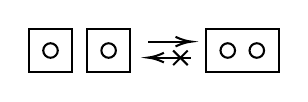
\begin{tikzpicture}[x=0.75pt,y=0.75pt,yscale=-0.7,xscale=0.7]
				%uncomment if require: \path (0,300); %set diagram left start at 0, and has height of 300
				%Shape: Square [id:dp8926747085287872] 
				\draw   (70,100) -- (100,100) -- (100,130) -- (70,130) -- cycle ;
				%Shape: Square [id:dp7911928154788817] 
				\draw   (110,100) -- (140,100) -- (140,130) -- (110,130) -- cycle ;
				%Shape: Circle [id:dp7972097445752802] 
				\draw   (80,115) .. controls (80,112.24) and (82.24,110) .. (85,110) .. controls (87.76,110) and (90,112.24) .. (90,115) .. controls (90,117.76) and (87.76,120) .. (85,120) .. controls (82.24,120) and (80,117.76) .. (80,115) -- cycle ;
				%Shape: Circle [id:dp2798464482392615] 
				\draw   (120,115) .. controls (120,112.24) and (122.24,110) .. (125,110) .. controls (127.76,110) and (130,112.24) .. (130,115) .. controls (130,117.76) and (127.76,120) .. (125,120) .. controls (122.24,120) and (120,117.76) .. (120,115) -- cycle ;
				%Straight Lines [id:da13754401873028943] 
				\draw    (152.11,108.89) -- (180,108.89) ;
				\draw [shift={(182,108.89)}, rotate = 180] [color={rgb, 255:red, 0; green, 0; blue, 0 }  ][line width=0.75]    (10.93,-3.29) .. controls (6.95,-1.4) and (3.31,-0.3) .. (0,0) .. controls (3.31,0.3) and (6.95,1.4) .. (10.93,3.29)   ;
				%Straight Lines [id:da986017380068096] 
				\draw    (154.11,119.89) -- (182,119.89) ;
				\draw [shift={(152.11,119.89)}, rotate = 0] [color={rgb, 255:red, 0; green, 0; blue, 0 }  ][line width=0.75]    (10.93,-3.29) .. controls (6.95,-1.4) and (3.31,-0.3) .. (0,0) .. controls (3.31,0.3) and (6.95,1.4) .. (10.93,3.29)   ;
				%Straight Lines [id:da5414382618735807] 
				\draw    (169.44,115) -- (179.44,125) ;
				%Straight Lines [id:da5354101657295061] 
				\draw    (169.44,125) -- (179.44,115) ;
				%Shape: Rectangle [id:dp9448845358260181] 
				\draw   (192,100) -- (242,100) -- (242,130) -- (192,130) -- cycle ;
				%Shape: Circle [id:dp5531546897679429] 
				\draw   (202,115) .. controls (202,112.24) and (204.24,110) .. (207,110) .. controls (209.76,110) and (212,112.24) .. (212,115) .. controls (212,117.76) and (209.76,120) .. (207,120) .. controls (204.24,120) and (202,117.76) .. (202,115) -- cycle ;
				%Shape: Circle [id:dp9053407831799309] 
				\draw   (222,115) .. controls (222,112.24) and (224.24,110) .. (227,110) .. controls (229.76,110) and (232,112.24) .. (232,115) .. controls (232,117.76) and (229.76,120) .. (227,120) .. controls (224.24,120) and (222,117.76) .. (222,115) -- cycle ;
			\end{tikzpicture}
		\end{minipage}
	\end{center}
	是满射, 但没有截面. 采用例 \ref{cohesion-family-of-sets} 对集合族的直观, 这就是说两个粘在一起的点无法分开 (右图).
	
	第二个例子是 $\mathsf {Fun}(B\mathbb{N},\mathsf {Set})$, 其中 $B\mathbb N$ 是将半群 $\mathbb N$ 视为单对象范畴. 这个范畴的对象是集合 $X$ 配备一个映射 $f\colon X\to X$. 态射
	\begin{center}
		\begin{minipage}
			{0.5\textwidth}
			% https://q.uiver.app/#q=WzAsNCxbMCwwLCJcXHswLDFcXH0iXSxbMSwwLCJcXHsqXFx9Il0sWzEsMSwiXFx7KlxcfSJdLFswLDEsIlxcezAsMVxcfSJdLFswLDFdLFsxLDJdLFswLDMsIjBcXG1hcHN0byAxXFxhdG9wIDFcXG1hcHN0byAwIiwyXSxbMywyXV0=
			\[\begin{tikzcd}[ampersand replacement=\&]
				{\{0,1\}} \& {\{*\}} \\
				{\{0,1\}} \& {\{*\}}
				\arrow[from=1-1, to=1-2]
				\arrow[from=1-2, to=2-2]
				\arrow["{0\mapsto 1\atop 1\mapsto 0}"', from=1-1, to=2-1]
				\arrow[from=2-1, to=2-2]
			\end{tikzcd}
			\]
		\end{minipage}
		\begin{minipage}
			{0.3\textwidth}
			\tikzset{every picture/.style={line width=0.75pt}} %set default line width to 0.75pt        
			\hspace{-2em}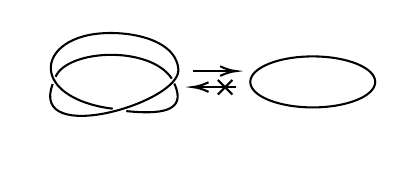
\begin{tikzpicture}[x=0.75pt,y=0.75pt,yscale=-0.7,xscale=0.7]
				%uncomment if require: \path (0,300); %set diagram left start at 0, and has height of 300
				%Curve Lines [id:da5256174669964437] 
				\draw    (57.33,121.78) .. controls (65.67,102.78) and (122.33,100.11) .. (137.33,123.11) ;
				%Curve Lines [id:da047957165101484955] 
				\draw    (55.33,126.78) .. controls (38.83,170.22) and (143.67,139.56) .. (141.83,116.67) .. controls (140,93.78) and (101,88.72) .. (80,93.11) .. controls (59,97.5) and (49.83,111.17) .. (55.83,123.17) .. controls (61.83,135.17) and (79.67,141.78) .. (96.67,143.78) ;
				%Curve Lines [id:da12392233177287926] 
				\draw    (106,145.44) .. controls (127.67,147.56) and (148.5,146.72) .. (139,126.44) ;
				%Shape: Ellipse [id:dp3575392941798332] 
				\draw   (191.33,125.33) .. controls (191.33,115.64) and (210.59,107.78) .. (234.33,107.78) .. controls (258.08,107.78) and (277.33,115.64) .. (277.33,125.33) .. controls (277.33,135.03) and (258.08,142.89) .. (234.33,142.89) .. controls (210.59,142.89) and (191.33,135.03) .. (191.33,125.33) -- cycle ;
				%Straight Lines [id:da8062516844631029] 
				\draw    (151.67,117.89) -- (179.56,117.89) ;
				\draw [shift={(181.56,117.89)}, rotate = 180] [color={rgb, 255:red, 0; green, 0; blue, 0 }  ][line width=0.75]    (10.93,-3.29) .. controls (6.95,-1.4) and (3.31,-0.3) .. (0,0) .. controls (3.31,0.3) and (6.95,1.4) .. (10.93,3.29)   ;
				%Straight Lines [id:da3938685457393487] 
				\draw    (153.67,128.89) -- (181.56,128.89) ;
				\draw [shift={(151.67,128.89)}, rotate = 0] [color={rgb, 255:red, 0; green, 0; blue, 0 }  ][line width=0.75]    (10.93,-3.29) .. controls (6.95,-1.4) and (3.31,-0.3) .. (0,0) .. controls (3.31,0.3) and (6.95,1.4) .. (10.93,3.29)   ;
				%Straight Lines [id:da45301762856536665] 
				\draw    (169,124) -- (179,134) ;
				%Straight Lines [id:da41762886315511905] 
				\draw    (169,134) -- (179,124) ;
			\end{tikzpicture}
		\end{minipage}
	\end{center}
	是满射, 但没有截面. 一个类似的例子是 $\operatorname{Sh}(S^1)$ 中 $S^1$ 的非平凡二重覆叠没有截面 (右图).
\end{example}

%
%\begin{proof}
%	假设\topos{} $\mathsf C$ 满足选择公理. 对任意满射 $p\colon X\to I$, 取截面 $s\colon I\to X$, 那么 $p^Y\colon X^Y\to I^Y$ 有截面 $s^Y\colon I^Y\to X^Y$, 从而 $X^Y\to I^Y$ 为满射, 即 $(-)^Y$ 保持满射.
%\end{proof}

\begin{prop}
	[label={IAC-technical-lemma}]
	{}
	假设\topos{} $\mathsf C$ 满足内蕴选择公理, 那么对其中任意满射 $f\colon Z\to X$, 都有 $\Pi_X(f) \to 1$ 是满射. 进一步, 记 $S=\Pi_X(f)$,
	则 $S^*Z\to S^*X$ (作为\topos{} $\mathsf C/S$ 中的映射, 定义见例 \ref{over-category-Sigma-adjunction}) 有截面.
\end{prop}

\begin{proof}
	回忆 $\Pi_X(f)$ 是 $f^X\colon Z^X\to X^X$ 沿 $\operatorname{id}_X\colon 1\to X^X$ 的拉回 (命题 \ref{pi-functor-absolute} 的证明), 而拉回保持满射 (命题 \ref{pullback-preserve-epis}), 故 $\Pi_X(f) \to 1$ 是满射. 映射 $S^*Z\to S^*X$ 的截面由取值映射 $S\times X\hookrightarrow Z^X\times X\overset{\operatorname{ev}}{\to} Z$ 给出.
\end{proof}

$\Pi_X(f)$ 是 ``$f$ 的截面的集合'', 所以内蕴选择公理是说满射在某种内蕴的意义上有截面.

\begin{prop}
	{(Diaconescu 定理)}
	满足内蕴选择公理的\topos{}一定是 Boole 的.
\end{prop}

\begin{proof}
	考虑任意子对象 $U\hookrightarrow X$. 由于单射是余核偶的等化子 (命题 \ref{topos-mono-regular}), 有 $U = \operatorname{eq}(X \rightrightarrows X \sqcup_U X)$. 我们的思路是考虑满射 $(X\sqcup X) \to (X\sqcup_U X)$ 的 ``截面'', 从而得到 $U\lor\neg U$.
	假设它有截面 $s\colon (X\sqcup_U X) \to (X\sqcup X)$, 如左图,
	\[\begin{tikzcd}[ampersand replacement=\&,column sep=small]
		V \& X \&\& {X\sqcup X} \& {1+1} \\
		\&\& {X\sqcup_U X}
		\arrow["t", from=1-4, to=1-5]
		\arrow["s"', hook, from=2-3, to=1-4]
		\arrow["{i_1}"{pos=0.7}, hook, from=1-2, to=2-3]
		\arrow["{si_1}"{pos=0.7}, shift left=2, hook', from=1-2, to=1-4]
		\arrow["{si_2}"'{pos=0.7}, hook', from=1-2, to=1-4]
		\arrow["{i_2}"'{pos=0.7}, shift right=2, hook, from=1-2, to=2-3]
		\arrow["f", from=1-1, to=1-2]
	\end{tikzcd}\quad
	\begin{tikzcd}[ampersand replacement=\&,column sep=small]
		V \& {X\sqcup X} \& {1+1} \\
		\& X
		\arrow["t",from=1-2, to=1-3]
		\arrow["{si_1f}", shift left=2, from=1-1, to=1-2]
		\arrow["f"', shift right=2, from=1-1, to=2-2]
		\arrow[from=1-2, to=2-2]
		\arrow["{si_2f}"', from=1-1, to=1-2]
	\end{tikzcd}\]
	那么 $s$ 为单射, 故对任何映射 $f\colon V\to X$, $f$ 等化 $i_1,i_2$ 当且仅当 $f$ 等化 $si_1,si_2$.
	而 $X\sqcup X \simeq X\times (1+1)$, 如右图,
	故 $f$ 等化 $si_1,si_2$ 等价于 $f$ 等化 $tsi_1,tsi_2$.
	这说明 $(U\hookrightarrow X)=\operatorname{eq}(tsi_1,tsi_2\colon X\rightrightarrows 1+1)$.
	
	由命题 \ref{IAC-technical-lemma}, 存在满射 $S\twoheadrightarrow 1$ 使得 $S^*(X\sqcup X)\to S^*(X\sqcup_U X)$ 有截面.
	
	\todo{}
	由于拉回是子对象 Heyting 代数的同态 (命题 \ref{subobject-lattice-Heyting-algebra}),
	
\end{proof}

另外, Bauer 的文章 (讲座) \cite{FSCM} 给出了 (外蕴) 选择公理推出排中律的一种证明.